%% Manuscript for Chaos: An Interdisciplinary Journal of Nonlinear Science (AIP Publishing), REVTeX 4.2.
%% Sources: sections/*.tex; figures/*.pdf (paper/chaos/make_figures_en.py); refs.bib (build_chaos.py).
%% Build: python paper/chaos/build_chaos.py  ->  manuscript.tex (single flattened file) and manuscript.pdf
\documentclass[aip,cha,reprint,amsmath,amssymb,longbibliography]{revtex4-2}

\usepackage{graphicx}
\usepackage{bm}
\usepackage{xcolor}
\usepackage[colorlinks=true,linkcolor=blue!55!black,citecolor=blue!55!black,urlcolor=blue!55!black]{hyperref}

% float placement: let LaTeX fill pages with figures instead of deferring them past the references
\renewcommand{\topfraction}{0.95}
\renewcommand{\bottomfraction}{0.8}
\renewcommand{\textfraction}{0.05}
\renewcommand{\floatpagefraction}{0.75}
\renewcommand{\dbltopfraction}{0.95}
\renewcommand{\dblfloatpagefraction}{0.75}
\setcounter{topnumber}{3}
\setcounter{bottomnumber}{2}
\setcounter{totalnumber}{5}
\setcounter{dbltopnumber}{3}

\newtheorem{proposition}{Proposition}
% text the author must supply before submission (printed in red)
\newcommand{\placeholder}[1]{\textcolor{red}{[#1]}}
% confidence interval in table cells, set smaller than the estimate
\newcommand{\ci}[2]{{\scriptsize[#1, #2]}}

\begin{document}

\title[Hidden attractors as a rare-event problem]{Searching for hidden attractors as a rare-event problem: An adaptive strategy portfolio with a worst-case guarantee}

\author{Maksim Elisov}
\email{maksimelisov2003@mail.ru}
\affiliation{Samara National Research University, Moskovskoye Shosse 34, Samara 443086, Russia}

\date{\today}

\begin{abstract}
An attractor is hidden if its basin does not intersect small neighborhoods of equilibria, so trajectories launched from unstable equilibria miss it; when the basin is also small, locating the attractor becomes rare-event detection in the space of initial conditions. We characterize a search method by its detection probability $P(N)$ after $N$ integrations and its cost $N_{0.9}$, relative to uniform sampling with $N_{0.9}\approx2.3/p$ for basin measure $p$. An adaptive method can gain only from what trajectories that miss the target reveal. We propose a portfolio of subset simulation driven by transient duration, active learning of basin boundaries, and a uniform share $\varepsilon$, and prove that it is at most $1/\varepsilon$ times costlier than uniform sampling while inheriting the scaling exponent of its splitting arm. On a four-level benchmark with a verification protocol, the portfolio reduces the cost of finding rare hidden attractors ($p\sim10^{-3}$--$10^{-2}$) by factors of 3--7. On a synthetic family, the cost scales as $p^{-0.45}$ down to $p=10^{-5}$, below which the time resolution of the transients limits it. On coupled copies of systems with hidden attractors, the gain in integrations reaches $10^3$--$10^4$. Measured in wall time, including against uniform sampling with recurrence-based early stopping, the gain persists for bounded trajectories (10--64 for a rare hidden regime of two coupled Chua circuits) but shrinks where trajectories escape quickly. The enumeration of regimes by the protocol reveals a hidden chaotic attractor of the coupled circuits born by the coupling. Documented failures stay within the guarantee.
\end{abstract}

\maketitle

\begin{quotation}
Some attractors of nonlinear systems are hidden: no trajectory started near an equilibrium ever reaches them, so the textbook way of finding attractors misses them. When such an attractor also has a tiny basin, finding it is like searching for a needle in a haystack of initial conditions, and published methods rarely report whether they beat random guessing. We recast the search as a rare-event problem and measure the cost of finding a target with a prescribed confidence. This makes methods comparable and shows that an advantage can come only from what unsuccessful trajectories reveal about the basins. On this basis, we build a search strategy that is guaranteed never to be much worse than random sampling, is several times better on typical problems, and is orders of magnitude better on rare targets in coupled systems, together with a benchmark and a protocol that catch numerical artifacts and transient chaos mistaken for attractors. Measured in computing time rather than in the number of trajectories, the advantage holds where trajectories stay bounded, as in typical physical systems.
\end{quotation}

\section{Introduction}\label{sec:intro}

An attractor is called hidden if its basin of attraction does not intersect small neighborhoods of equilibria; otherwise, the attractor is self-excited.\cite{LeonovKuznetsov2013,Leonov2011PLA,Kuznetsov2020JCSSI} Hidden oscillations occur in Chua circuits,\cite{Leonov2012PhysD,Stankevich2017,Kuznetsov2023Chua} in control systems with saturation,\cite{Andrievsky2017Aircraft} in the Aizerman and Kalman problems,\cite{Bragin2011} in generalized Lorenz and Rabinovich systems,\cite{Chen2017OnePath,Kuznetsov2018Rabinovich,Kuznetsov2020Lorenz} in systems without equilibria,\cite{JafariSprottGolpayegani2013,Wei2011} with a single stable equilibrium,\cite{WangChen2012,Molaie2013} with lines and surfaces of equilibria,\cite{JafariSprott2013,Jafari2016Surfaces} in two-dimensional maps,\cite{Jiang2016Maps,WangDing2018Map,Huynh2019} and in neural network models.\cite{DancaKuznetsov2017Hopfield} Reviews\cite{Dudkowski2016,JafariSprottNazarimehr2015,GuanXie2025} show that the number of such examples has grown by orders of magnitude over the past fifteen years. Since a hidden attractor usually coexists with other attractors, searching for it is a problem of multistable dynamics.\cite{Feudel2008,PisarchikFeudel2014} Attractors whose basins occupy a small fraction of the state space are called rare.\cite{Chudzik2011Rare,Yue2021RareDuffing}

The main practical difficulty stems from the definition itself. The standard procedure for finding attractors launches trajectories from neighborhoods of unstable equilibria along their unstable manifolds. By definition, this procedure does not find a hidden attractor, and with an unlucky choice of initial conditions, such an attractor is easily missed. Analytical--numerical methods have been proposed for localizing hidden attractors: harmonic balance and the describing function followed by continuation in a parameter.\cite{Leonov2011PLA,KuznetsovLeonovVagaitsev2010,Kuznetsov2017IFAC} There are also geometric heuristics: perpetual points,\cite{Prasad2015,Dudkowski2015PP,Dudkowski2017PP} connecting curves\cite{Gilmore2010CC,GuanXie2021CC,Naseri2021} and surfaces,\cite{Song2023CS} coordinate-wise zero-velocity sets,\cite{Godara2018CVS} and parameter switching.\cite{Danca2018Switching} Evolutionary search over initial conditions is used as well.\cite{Zelinka2016,Zelinka2021Chapter} A general tool is the estimation of basins by sampling initial conditions,\cite{Menck2013,DatserisWagemakers2022,Datseris2023Framework,StenderHoffmann2022,Gelbrecht2020MCBB} together with set-oriented methods.\cite{Hsu1987,DellnitzHohmann1997} A sample of $n$ initial conditions detects an attractor of basin fraction $p$ with probability $1-(1-p)^n$,\cite{Datseris2023Framework} so rare attractors are found either by very large samples or by continuation from parameter values where they are not rare: path following combined with basin stability\cite{Brzeski2017} and global continuation, which seeds the search at each parameter value with the attractors found at the previous one.\cite{Datseris2023Framework,Datseris2026Global,Haerter2026BBT} The limitations of the heuristics are well known. Perpetual points may not exist at all, or they may lead to something other than the target.\cite{Nazarimehr2017PP,Jafari2015LimitPP,Jafari2026NoPP} Connecting curves do not always pass through the basin of the hidden attractor.\cite{GuanXie2025}

Assessments of localization methods almost always remain qualitative: ``the attractor was found from such-and-such a point.'' How many integrations were needed, with what probability the method finds the target within a given budget, and how much better it is than uniform sampling are usually not reported. This picture emerges from the review in Ref.~\onlinecite{GuanXie2025} and from an analysis of the full text of Ref.~\onlinecite{Zelinka2016}. Meanwhile, hiddenness and rarity are different properties. In well-known examples, the basin of a hidden attractor often occupies most of the natural region of initial conditions; for the Rabinovich system at $r=100$, it occupies 76\% (Sec.~\ref{sec:bench}). What makes the problem hard is a small basin measure $p$, not the absence of a connection to equilibria. In addition, a long-lived transient chaotic set is sometimes declared a ``hidden attractor.'' Examples are the story of the ``hidden attractor'' of the classical Lorenz system\cite{Munmuangsaen2018,SprottMunmuangsaen2018Comment} and the Rabinovich--Fabrikant system;\cite{Danca2016Transient} see also Refs.~\onlinecite{YorkeYorke1979,GrebogiOttYorke1983,LaiTel2011}. Comparing methods therefore requires an explicit verification protocol.

If the target basin is small, finding the attractor becomes the problem of detecting a rare event in the space of initial conditions. Well-developed tools exist for such problems. They include multilevel splitting\cite{Glasserman1999,CerouGuyader2007,Cerou2019AMS} and its static counterpart, subset simulation,\cite{AuBeck2001} the cross-entropy method,\cite{Rubinstein1999CE} and sequential design of experiments with active learning of the failure domain.\cite{Bect2012,Echard2011AKMCS} Novelty search and quality-diversity algorithms belong here as well.\cite{LehmanStanley2011,MouretClune2015,Pugh2016QD,CullyDemiris2018} Rare-event algorithms have been applied, for example, to extreme events and transitions in climate models\cite{Ragone2018,Lestang2018TAMS} and to high-dimensional dynamical systems.\cite{Baars2021AMS} Machine-learning methods for basins of attraction\cite{Wang2022HAL,Cao2025AL,Yang2024PRR,DNNBasins2021,Gameiro2025,Haerter2026BBT} estimate the fractions of already known basins rather than search for unknown attractors. To the best of our knowledge, these tools have not been applied systematically to the search for hidden attractors.

The contributions of this work are as follows.
\begin{enumerate}
\item The search for a hidden attractor is formulated as a rare-event detection problem. The quality of a method is measured by the detection probability $P(N)$ as a function of the budget $N$, by the cost $N_{0.9}$, by the gain factor $G$ relative to uniform sampling, and by the scaling exponent $s$ in $N_{0.9}\propto p^{-s}$. We identify three channels of information through which an adaptive method can outperform uniform sampling at all.
\item We build a four-level benchmark: three-dimensional flows, maps, four-dimensional systems, and synthetic families with analytically known basin measure. We develop a protocol for identifying and verifying attractors. While refining it, we found a numerical artifact in the Chua circuit and a discrepancy with a published table of basin fractions.
\item We propose a portfolio of adaptive strategies: multilevel splitting driven by transient duration, active learning of basin boundaries, and a uniform share. We prove that in the worst case it is at most $1/\varepsilon$ times costlier than uniform sampling and inherits the scaling exponent of the splitting arm. We construct a cost model with diagnostics that predict when a gain is possible.
\item We measure the gain and its scaling with basin measure and dimension, and we measure the cost not only in integrations but in integrator steps and wall time, against uniform sampling with the same evaluation and against uniform sampling with recurrence-based early stopping (Attractors.jl). The gain carries over to time where trajectories are bounded and shrinks where most of them escape quickly. On two coupled Chua circuits, a rare hidden regime ($p=2\times10^{-5}$) is found 55 times faster in integrations and 10--64 times faster in time, and the enumeration of regimes by the identification protocol reveals a hidden chaotic attractor of the coupled circuits that is born by the coupling and that we have not found reported. Failure cases, including the limit set by the time resolution of the reaction coordinate, are documented explicitly; enlarged regions of initial conditions and continuation in a parameter do not make the hidden attractors of the benchmark rare.
\end{enumerate}

\section{Problem formulation}\label{sec:problem}

\subsection{Hidden attractors}\label{sec:hidden}

Consider an autonomous system in $\mathbb{R}^n$: a flow $\dot x=F(x)$ or a map $x_{k+1}=F(x_k)$ with a smooth (or piecewise-smooth) right-hand side. Let $A$ be an attractor, $W(A)$ its basin, and $\mathcal{E}$ the set of equilibria (fixed points). The attractor $A$ is \emph{self-excited} if there exists $e\in\mathcal{E}$ such that $W(A)\cap U_\varepsilon(e)\neq\varnothing$ for every $\varepsilon>0$; otherwise, $A$ is \emph{hidden}.\cite{LeonovKuznetsov2013} Three consequences matter for the search. Trajectories launched from neighborhoods of equilibria do not reach a hidden attractor. In systems without equilibria and in systems with a single stable equilibrium, all nontrivial attractors are hidden. A hidden attractor may coexist with self-excited ones, and then its basin is an ``island'' that the unstable manifolds of the equilibria do not reach.

A continuous characteristic complements the binary definition. Let $\nu_\varepsilon$ be the uniform distribution on the union of the $\varepsilon$-neighborhoods of the equilibria (in an extended version, also on the $\varepsilon$-tubes around their unstable manifolds). We call
\begin{equation}
h_\varepsilon(A)=\Pr_{x\sim\nu_\varepsilon}\bigl[x\in W(A)\bigr]
\label{eq:heps}
\end{equation}
the \emph{hiddenness measure}. For a hidden attractor and a finite set of equilibria, $h_\varepsilon(A)=0$ for all sufficiently small $\varepsilon$, and the function $\varepsilon\mapsto h_\varepsilon$ shows the ``depth'' of hiddenness; for a continuum of equilibria, a common $\varepsilon$ is not guaranteed, and for systems without equilibria we set $h_\varepsilon=0$. A measured $h_\varepsilon=0$ is a necessary condition of hiddenness, not a sufficient one: it bounds the measure of $W(A)\cap U_\varepsilon(\mathcal E)$ from above by the sampling resolution. Below, it is measured for the benchmark systems (Sec.~\ref{sec:protocol}).

\subsection{Search as rare-event detection}\label{sec:rare}

Let $B\subset\mathbb{R}^n$ be a compact region of initial conditions with normalized Lebesgue measure $\mu$, $\mu(B)=1$. The target attractor $A^*$ has a basin $W^*$ of measure $p=\mu(W^*\cap B)\ll1$. The unit of cost is one integration of standard length $T=T_{\rm tr}+T_{\rm obs}$ (a transient segment and an observation window); for maps, it is one orbit. Below, one integration of one initial condition is also called one \emph{evaluation}. An algorithm $\mathcal{A}$ chooses initial points $x_1,x_2,\dots\in B$ adaptively: the point $x_k$ may depend on the results of the previous integrations. Let $\tau=\min\{k: x_k\in W^*\}$ be the index of the first hit. The quality of the algorithm is described by the detection probability and by the cost at confidence level $1-\delta$:
\begin{equation}
\begin{split}
&P_{\mathcal A}(N)=\Pr[\tau\le N],\\
&N_{1-\delta}(\mathcal A)=\min\{N: P_{\mathcal A}(N)\ge 1-\delta\}.
\end{split}
\label{eq:pn}
\end{equation}
The probability is taken over the internal randomness of the algorithm; throughout, $\delta=0.1$. The reference point is uniform independent sampling:
\begin{equation}
\begin{split}
&P_0(N)=1-(1-p)^N,\\
&N^0_{1-\delta}=\left\lceil\frac{\ln\delta}{\ln(1-p)}\right\rceil\approx\frac{\ln(1/\delta)}{p},\qquad N^0_{0.9}\approx\frac{2.3}{p}.
\end{split}
\label{eq:uniform}
\end{equation}
The gain factor $G_{1-\delta}(\mathcal A)=N^0_{1-\delta}/N_{1-\delta}(\mathcal A)$ is equivalent to an ``effective basin measure'' $p_{\rm eff}=pG$. On families with a controlled basin measure, we measure the scaling exponent $s$ in $N_{0.9}\propto p^{-s}$; for uniform sampling, $s=1$. A method has an \emph{order-of-growth gain} if $s<1$ with statistical significance and a \emph{constant-factor gain} if $s\approx1$ but $G>1$. A hit counts only if the candidate passes the identification and verification protocol of Sec.~\ref{sec:protocol}; transient chaos mistaken for an attractor is a failure of the method.

\subsection{Where a gain can come from}\label{sec:channels}

If an algorithm receives only the target indicator of each point, adaptivity cannot help in the worst case. Partition $B$ into $\lfloor1/p\rfloor$ cells of measure $p$ and let $W^*$ be a cell chosen uniformly at random. An algorithm that learns only whether $x_k\in W^*$ excludes at most one cell per query, so $\Pr[\tau\le N]\le Np$ and $N_{1-\delta}\ge(1-\delta)/p$ for every algorithm; uniform sampling is therefore within the factor $\ln(1/\delta)/(1-\delta)\approx2.6$ of the optimum. A gain is possible only through the information carried by the trajectories that did \emph{not} land in $W^*$. Among the sources of such information that cost one integration per point, we distinguish three channels (information about the vector field that needs no integration, such as harmonic balance or Lyapunov functions, is outside this setting).
\begin{itemize}
\item \textbf{Channel A: basin geometry.} Labels are spatially correlated. If the target basin adjoins already found boundaries between known basins, sampling near these boundaries is enriched with the target.
\item \textbf{Channel B: transients.} Trajectories converging to known attractors or escaping to infinity carry information about proximity to unseen invariant sets: the escape time, delays near saddles, and the mismatch between the early segment of a trajectory and its asymptotic regime. Near a basin boundary, a trajectory follows for a long time the stable manifold of the invariant set on the boundary (the edge state\cite{Skufca2006Edge,Schneider2007Edge,Vollmer2009Edge}), and its transient lengthens. Invariant sets on basin boundaries are classically located by straddle (bisection) methods that exploit exactly this effect,\cite{NusseYorke1989} and long transients are the signal of the stagger-and-step method for finding chaotic saddles.\cite{SweetNusseYorke2001}
\item \textbf{Channel C: prior sets.} Classical heuristics (nullclines, perpetual points, connecting curves) define a distribution of starting points that may be enriched with the target.
\end{itemize}
The proposed method (Sec.~\ref{sec:method}) uses all three channels. The cost model (Sec.~\ref{sec:costmodel}) indicates which channel works for which basin properties and provides an observable diagnostic.

\section{Benchmark and identification protocol}\label{sec:bench}

\subsection{Levels of the benchmark}\label{sec:levels}

The benchmark is designed to separate two properties, hiddenness and rarity, and to test the method on all types of systems for which heuristics have been proposed. Equations, parameters, and integration settings are given in Appendix~\ref{app:systems}, and a summary is given in Table~\ref{tab:benchmark}. A gallery of level-A attractors is shown in Fig.~\ref{fig:gallery3d}.
\begin{itemize}
\item \textbf{Level A: three-dimensional flows.} The Chua circuit with two parameter sets\cite{Leonov2011PLA,GuanXie2025,Kuznetsov2023Chua} (Fig.~\ref{fig:chuaII} and Appendix~\ref{app:systems}). Systems without equilibria: NE4, Wang--Chen \#1, and Wei,\cite{Wei2011,JafariSprottGolpayegani2013} as well as the 2026 system of Jafari \textit{et al.} without fixed and perpetual points.\cite{Jafari2026NoPP} Systems with a single stable equilibrium: Wang--Chen \#2, SE3, and SE11.\cite{WangChen2012,Molaie2013} The LE1 system with a line of equilibria\cite{JafariSprott2013} and the Rabinovich system.\cite{Kuznetsov2018Rabinovich} The negative controls are the transient chaos of the Lorenz system at $(a,r,b)=(4,29,2)$\cite{YorkeYorke1979} and the ``hidden attractor'' of the Rabinovich system at $r=6.8$, which, according to Ref.~\onlinecite{SprottMunmuangsaen2018Comment}, is a transient set.
\item \textbf{Level B: maps.} The map of Huynh \textit{et al.} without fixed points.\cite{Huynh2019} Eight cases of the general family of Jiang \textit{et al.}:\cite{Jiang2016Maps} four without fixed points and four with a single stable one. Three parameter sets of the same family in the form of Ref.~\onlinecite{Ouannas2018}. The H\'enon map serves as a control. Phase--basin portraits of the maps and of the other systems are given in Appendix~\ref{app:systems}.
\item \textbf{Level C: four-dimensional systems.} The simplified Lorenz system of Li and Sprott without equilibria\cite{LiSprott2014} in three regimes (a torus and a pair of strange attractors; a cycle and a pair; hyperchaos) and the system of Jahanshahi \textit{et al.}\cite{Jahanshahi2019} This level is used for the census and the verification protocol; the search experiments are run on levels A, B, and D.
\item \textbf{Level D: synthetic families} with analytically known basin measure (Sec.~\ref{sec:synth}).
\end{itemize}

The region $B$ for three-dimensional systems is the cube $[-10,10]^3$, the natural region of the original publications. For the Chua circuit, we take the box $[-10,10]^2\times[-15,15]$ proposed in Ref.~\onlinecite{Zelinka2016}. For NE4 and the Rabinovich system, the region is twice the extent of the attractor. Basin fractions are estimated from $5\times10^4$ uniform points for level A and $2\times10^4$ for the other levels; for the Chua circuit, they were checked by an independent computation in Attractors.jl.\cite{Datseris2018JOSS,DatserisWagemakers2022}

Table~\ref{tab:benchmark} confirms that hiddenness and rarity are different properties. In the Rabinovich system and in Wang--Chen \#2, the hidden attractor occupies 76\% and 67\% of the region. Only the targets of Chua~II, SE11, LE1, the Jafari cycle and chaos, and the Huynh map are rare ($p<10^{-2}$). The Jiang maps, which Ref.~\onlinecite{Jiang2016Maps} characterizes as having ``tiny'' basins, give $p\approx0.03$--$0.10$ in boxes around the attractor. The classical heuristics behave on this benchmark as described in the review in Ref.~\onlinecite{GuanXie2025}, and none of them helps on the rare targets (Appendix~\ref{app:classic}). The literature baseline for the search experiments is differential evolution (DE) over initial conditions with the cost function of Ref.~\onlinecite{Zelinka2016}, which, unlike our strategies, is given the size of the target (Appendix~\ref{app:ablation}).

\begin{table*}
\caption{Benchmark: search targets (hidden attractors), basin measures $p$ in the region $B$, and the cost of uniform sampling $N^0_{0.9}$. Basin measures are from the uniform census ($5\times10^4$ points for level A, $2\times10^4$ otherwise); $N^0_{0.9}$ is the 0.9 quantile of the first-hit index over $R=50$ runs of uniform sampling ($R=20$ for the Jafari chaos; for the nonrare targets, it is $\lceil\ln0.1/\ln(1-p)\rceil$). A slash separates two symmetric attractors, a semicolon separates different targets, and ``both'' means the cost of hitting either of the two; the search tables of Sec.~\ref{sec:results} use the combined measure of the two symmetric attractors and remeasure $N^0_{0.9}$ with their own runs. $\lambda$ is the largest Lyapunov exponent.}
\label{tab:benchmark}
\footnotesize
\setlength{\tabcolsep}{4pt}
\begin{ruledtabular}
\begin{tabular}{llllrr}
Level & System & Equilibria & Target & $p$ & $N^0_{0.9}$ \\
\hline
A & Chua I & F$_0$ stable, F$_\pm$ saddle-foci & two chaotic (A, B) & 0.017 / 0.018 & 136 / 124 \\
 & Chua II & F$_0$ saddle-focus, F$_\pm$ stable & cycle LC; two chaotic & 0.992; 0.0014 / 0.0013 & 1; 772 (both) \\
 & NE4 & none & chaos ($\lambda\approx0.03$) & 0.33 & 6 \\
 & Wang--Chen \#1 & none & chaos & 0.103 & 22 \\
 & Wei (NE2) & none & chaos & 0.096 & 23 \\
 & Jafari 2026, $a_3=-1$ & none; no perpetual points & cycle & 0.009 & 229 \\
 & Jafari 2026, $a_3=-3.548$ & none & fragile chaos ($\lambda\approx0.05$) & $(2$--$5)\times10^{-4}$ & 5331 \\
 & Wang--Chen \#2 & one, stable & chaos & 0.666 & 3 \\
 & SE3 & one, stable & chaos & 0.153 & 14 \\
 & SE11 & one, stable & chaos & 0.0079 & 302 \\
 & LE1 & line $x=y=0$ & chaos & 0.0016 & 1422 \\
 & Rabinovich, $r=100$ & saddle at 0, two stable foci & chaos & 0.763 & 2 \\
\hline
B & Huynh 2019 & none & chaos & 0.0091 & 211 \\
 & Jiang 2016, NF I e, f, g, i & none & chaos & 0.028--0.039 & 59--82 \\
 & Jiang 2016, SF I a--d & one, stable & chaos & 0.065--0.10 & 22--37 \\
\hline
C & Li--Sprott 4D, $a=6$ & none & torus; two strange & 0.090; 0.446 / 0.464 & 25; 4 \\
\hline
D & D1, D2 (base SE3), $n=4$--14 & as for the base & chaos of the base & $10^{-2}$--$10^{-7}$ & 258--$2.1\times10^{7}$ \\
\end{tabular}
\end{ruledtabular}
\end{table*}

\begin{figure*}
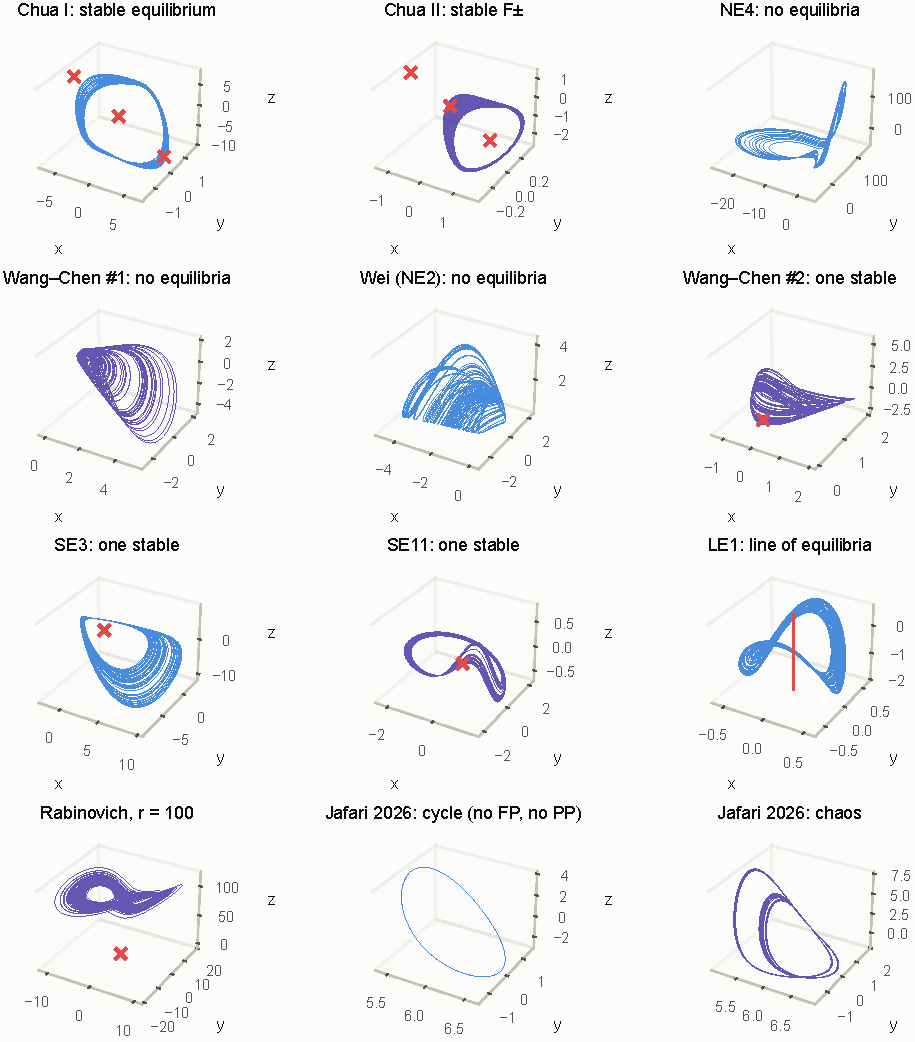
\includegraphics[width=\textwidth]{figures/fig32_gallery_3d.pdf}
\caption{Hidden attractors of the level-A benchmark. Crosses mark equilibria; for LE1, the red line is the line of equilibria $x=y=0$. NE4, Wang--Chen \#1, Wei, and the Jafari 2026 system have no equilibria, and in Wang--Chen \#2, SE3, and SE11 the single equilibrium is stable, so all attractors shown are hidden by definition.}
\label{fig:gallery3d}
\end{figure*}

\begin{figure*}
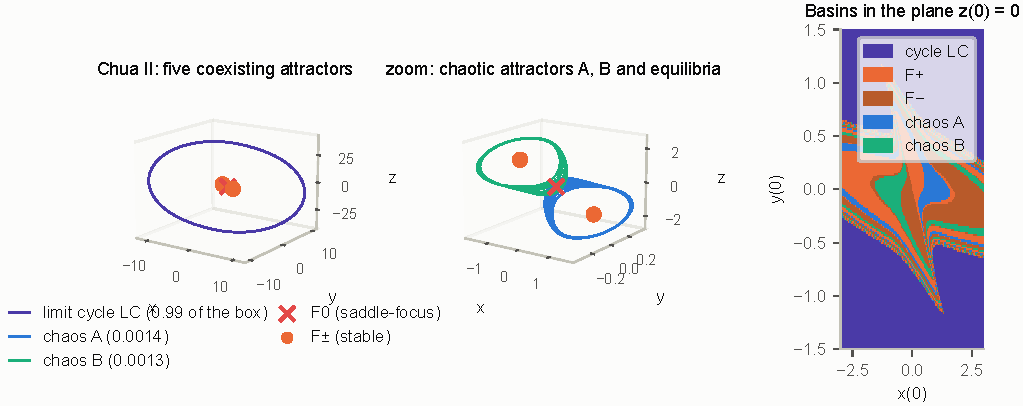
\includegraphics[width=\textwidth]{figures/fig31_chua_II_coexisting.pdf}
\caption{Chua circuit, parameter set II: five coexisting attractors. (a) The large limit cycle LC (basin fraction in the box 0.992), the chaotic attractors A and B (0.0014 and 0.0013), the saddle-focus F$_0$, and the stable foci F$_\pm$. (b) Enlarged fragment; the chaotic attractors surround F$_\pm$. (c) Basins in the plane $z(0)=0$ (window $|x|\le3$, $|y|\le1.5$, axes not to scale). The basins of the chaotic attractors are narrow strips between the basins of F$_\pm$ and of the cycle; a search can exploit only these boundaries and the long transients near them.}
\label{fig:chuaII}
\end{figure*}

\subsection{Synthetic families with known basin measure}\label{sec:synth}

To measure the scaling of the cost for $p$ down to $10^{-7}$ and dimensions up to 14, the three-dimensional system SE3 with a hidden attractor ($p_W=0.153$ in $[-10,10]^3$, where $W_{\rm HA}$ denotes its basin) is embedded in $\mathbb{R}^{3+m}$. The search region is $B=[-10,10]^3\times[-1,1]^m$. We use two constructions with opposite properties: D1 has no transient signal, and D2 has a signal on all scales.

\textbf{D1, ``embedding with a gate.''} The system is
\begin{equation}
\begin{split}
&\dot x=F(x)-g(w)\,(x-e),\qquad \dot w=-\kappa w,\\
&g(w)=\frac{H}{1+\exp\bigl(-400(|w|-\rho)/\rho\bigr)},
\end{split}
\label{eq:d1}
\end{equation}
where $e$ is the stable equilibrium of the base, $H=50$, and $\kappa=0.5$. While $|w|>\rho$, the ``gate'' pulls $x$ toward $e$. Therefore, the basin of the hidden attractor is approximately $W_{\rm HA}\times\{|w_0|\le\rho\}$, and
\begin{equation}
p(\rho,m)=p_W\,\frac{V_m(\rho)}{2^m},\qquad V_m(\rho)=\frac{\pi^{m/2}\rho^m}{\Gamma(m/2+1)}.
\label{eq:pD}
\end{equation}
The measured fractions agree with Eq.~\eqref{eq:pD} within 5\%--15\%. Outside a thin rim of the ball, the transient hardly depends on $|w_0|$, so channel B is practically absent in D1.

\textbf{D2, ``edge state.''} Here, the embedding is decoupled:
\begin{equation}
\dot x=F(x),\qquad \dot w=\kappa\, w\,\bigl(|w|^2/\rho^2-1\bigr),\qquad \kappa=1.
\label{eq:d2}
\end{equation}
The sphere $|w|=\rho$ is repelling. For $|w_0|<\rho$, the coordinates $w$ decay and $x$ follows the base; for $|w_0|>\rho$, the norm $|w|$ blows up in finite time. The target basin is exactly $W_{\rm HA}\times\{|w_0|<\rho\}$, and formula~\eqref{eq:pD} is exact given $p_W$; a check gave $p_{\rm meas}=0.00102$ and $0.00100$ at $p=0.001$. The escape time for $|w_0|=\rho(1+\Delta)$ equals $\ln\bigl((1+\Delta)^2/((1+\Delta)^2-1)\bigr)/(2\kappa)\approx\ln(1/2\Delta)/(2\kappa)$ for small $\Delta$. It diverges at the basin boundary (Fig.~\ref{fig:d2mech}), as for edge states of real systems.\cite{Vollmer2009Edge,LucariniBodai2017} In D2, channel B is informative on all scales down to the integration step.

\begin{figure*}
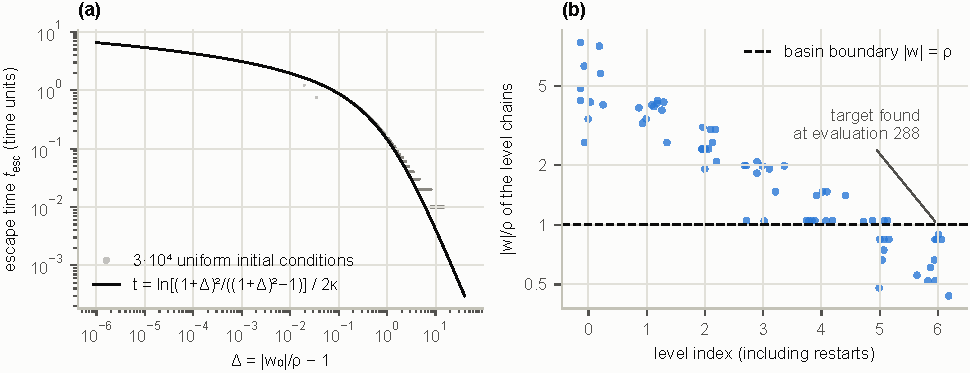
\includegraphics[width=\textwidth]{figures/fig37_d2_mechanism.pdf}
\caption{Mechanism of the splitting gain in family D2 ($n=6$, $p=10^{-4}$). (a) Escape time versus the relative distance to the basin boundary $\Delta=|w_0|/\rho-1$; dots are $3\times10^4$ uniform initial conditions, and the line is the exact law $\ln\bigl((1+\Delta)^2/((1+\Delta)^2-1)\bigr)/(2\kappa)$. The steps on the right reflect the discreteness of the integration step. (b) $|w|/\rho$ for the seeds of the chains over the levels of one run; the chains contract to the ball $|w|<\rho$, and the target is found after 288 integrations, whereas uniform sampling needs $N^0_{0.9}=1.7\times10^4$.}
\label{fig:d2mech}
\end{figure*}

\subsection{Identification and verification protocol}\label{sec:protocol}

\textbf{Trajectory fingerprint.} A trajectory is integrated by the fourth-order Runge--Kutta method (RK4) with a fixed step (maps are iterated) over the transient segment $T_{\rm tr}$ and the observation window $T_{\rm obs}$. Escape is detected by the condition $|x|>R_{\rm esc}$. On the observation window, we compute the largest Lyapunov exponent $\lambda$ by the two-trajectory method,\cite{Benettin1980} the mean speed, the maximum norm, the frequency of local maxima, the amplitude contraction ratio, and the coordinate-wise mean, standard deviation, minimum, and maximum. The same statistics are computed on an early window; they are needed by the reaction coordinate (Sec.~\ref{sec:xi}). The kernels are implemented in Numba\cite{Lam2015Numba} and compute the fingerprints inside the integrator, at about $3\times10^8$ RK4 steps per second on 14 cores.

\textbf{Templates and matching.} The template of a regime is the mean $\mu$ and spread $\sigma$ of the fingerprint over 64 copies. The copies start from random points of a trajectory segment on the attractor of length $4T_{\rm obs}$ (phase randomization) with relative noise $10^{-3}$. A trajectory with fingerprint $f$ is assigned to the template with the smallest
\begin{equation}
z=\max_i\frac{|f_i-\mu_i|}{\sigma_i+0.02\,(1+|\mu_i|)},
\label{eq:z}
\end{equation}
provided that $z<6$ and the classes are compatible: a chaotic template requires $\lambda>0.005$, and a regular one requires $\lambda<0.02$; in the overlap, the fingerprint decides. Converged trajectories are compared with equilibria by their final point with tolerance $10^{-3}L$, where $L$ is half the largest edge of $B$. Decaying trajectories ($\lambda<-0.002$ and amplitude contraction) are compared by the center of the window. Unmatched trajectories are clustered (DBSCAN), and a new template is calibrated for each cluster; this is how unknown regimes are discovered, during a search as well as in the enumeration of the regimes of a new system.

\textbf{Verification.} Each candidate passes four checks: the lifetime (the integration is continued for at least 20 windows and, for claims of a chaotic attractor, up to $10^4$--$10^5$ time units), convergence in the step (the same template and stable basin fractions under $\Delta t\to\Delta t/2$), an independent integrator (DOP853\cite{Hairer1993} with $\mathrm{rtol}=10^{-11}$ and Attractors.jl with Vern9), and the sign of the Lyapunov exponent over consecutive windows. For claims of hiddenness, $h_\varepsilon$ is estimated by sampling in the $\varepsilon$-neighborhoods of all equilibria and along their unstable manifolds, $\varepsilon\in\{10^{-3},10^{-2},10^{-1}\}L$; it distinguishes deeply hidden attractors (SE3, SE11) from shallowly hidden ones (Chua~I, the Rabinovich system), and the number of starts bounds its resolution (Appendix~\ref{app:verification}). The protocol was refined on three cases that change the conclusions if missed (Appendix~\ref{app:verification}): a numerical ``transient chaos'' of the Chua circuit at $\Delta t=0.01$, which underestimates the fractions of the hidden attractors almost twofold; a published table of basin fractions whose hidden-attractor fractions coincide with ours only at that coarse step; and intermittency and long-lived transient sets mistaken for attractors. The step-convergence and lifetime checks are therefore mandatory.

\section{Method}\label{sec:method}

The method is a portfolio of three arms: multilevel splitting driven by transient duration (channel B), active learning of basin boundaries (channel A), and a uniform share that bounds the worst case. Prior sets (channel C) enter as a distribution of starting points and candidates. All arms receive, for each point, only its fingerprint and the label produced by the protocol of Sec.~\ref{sec:protocol}. The strategies do not know which label is the target. Two configurations are used below: the \emph{portfolio with full integration}, with which the gains in integrations of Sec.~\ref{sec:rare_ab}--\ref{sec:coupled} are measured, and the \emph{portfolio with two-stage evaluation} of Sec.~\ref{sec:twostage}, with which the costs in steps and wall time of Sec.~\ref{sec:cost} are measured.

\subsection{Reaction coordinate: transient duration}\label{sec:xi}

For an initial point $x_0$ with a trajectory fingerprint, we define
\begin{equation}
\xi(x_0)=\begin{cases}\dfrac{\ln k_{\rm esc}}{\ln N_{\rm tot}}\in[0,1], & \text{escape at step } k_{\rm esc},\\[2mm] 1+D(x_0), & \text{bounded trajectory},\end{cases}
\label{eq:xi}
\end{equation}
where
\begin{equation*}
D=\frac{\bigl\|(m_{\rm early}-m_{\rm obs},\ s_{\rm early}-s_{\rm obs})\bigr\|}{L}.
\end{equation*}
Here, $k_{\rm esc}\in\{1,\dots,N_{\rm tot}\}$ is the integration step at which the trajectory left the escape radius, $N_{\rm tot}$ is the number of integration steps, and $m$ and $s$ are the coordinate-wise means and standard deviations over the early window (the first steps of the transient segment) and over the observation window; all trajectories that escape at the first step share the value $\xi=0$. A trajectory that quickly settles onto its regime has $D\approx0$. A trajectory that lingers near an edge state on a basin boundary has a large $D$ or a large $k_{\rm esc}$. In rare-event algorithms, the levels are defined by a score (importance) function, and the optimal score is the committor, the probability of reaching the target before the alternatives.\cite{Lestang2018TAMS,Lucente2022Committor} The committor is unknown here; $\xi$ is a cheap proxy computed from a single trajectory that does not use the target label. The coordinate is built on transient rather than asymptotic features because only the former carry a signal (Appendix~\ref{app:diagnostics}): on uniform samples, transient features separate the points near the target basin from the rest with an area under the receiver operating characteristic curve (AUC) of 0.88--0.97, whereas asymptotic features (the Lyapunov exponent, the range) reach only 0.5--0.75.

\subsection{Multilevel splitting in the space of initial conditions}\label{sec:sus}

For the static problem ``initial condition $\to$ fingerprint,'' the static counterpart of adaptive multilevel splitting\cite{CerouGuyader2007} is subset simulation;\cite{AuBeck2001} below, we call it splitting. Levels are set adaptively by a quantile of $\xi$, and the sample above a level is replenished by conditional Markov chains. The algorithm is as follows.
\begin{enumerate}
\item Reference sample: $n_0=50$ uniform points of $B$.
\item The level $\xi_l$ is the value of $\xi$ at the $(n_0p_0)$th largest point, $p_0=0.2$. These $n_0p_0=10$ points are the seeds of the chains.
\item Each chain makes $1/p_0-1=4$ random-walk steps $y=x+\sigma(b-a)\eta$, $\eta\sim\mathcal{N}(0,I)$, with mirror reflection into the parallelepiped $B=[a,b]$. A step is accepted if $\xi(y)\ge\xi_l$; a rejected proposal leaves the chain in its current state, which is counted again as a state of the level. Every proposal costs one integration, so a level costs $n_0(1-p_0)=40$ integrations. For the uniform measure on $B$, a symmetric proposal with reflection, and a fixed $\sigma$, this is the Metropolis algorithm for the conditional distribution on $\{\xi\ge\xi_l\}$.
\item The step $\sigma$ (initial value 0.1) is adapted to the acceptance rate, a simple variant of adaptive proposal scaling in subset simulation:\cite{Papaioannou2015} below an acceptance rate of 0.2, it is halved; below 0.4, it is divided by 1.25; above 0.6, it is multiplied by 1.5.
\item The next level is chosen from all states of the chains of the current level (step 2). On stagnation (a relative increase of the level below 2\% or $\sigma<0.005$) for two levels, and also after 10 levels, the algorithm restarts with a new uniform reference sample.
\end{enumerate}
Restarts protect against the case in which the chains have contracted onto a nontarget region with a long transient. In the benchmark, we compared three coordinates: $\xi$ from Eq.~\eqref{eq:xi}, the escape step alone, and the multidimensional ``rarity'' of the fingerprint (the mean distance to the $k=5$ nearest neighbors in the reference sample). Figure~\ref{fig:suschains} shows how the chains of two levels are distributed over the basin map of a Jiang map, and Fig.~\ref{fig:d2mech} shows how the chains in D2 contract to the ball $|w|<\rho$.

\begin{figure}
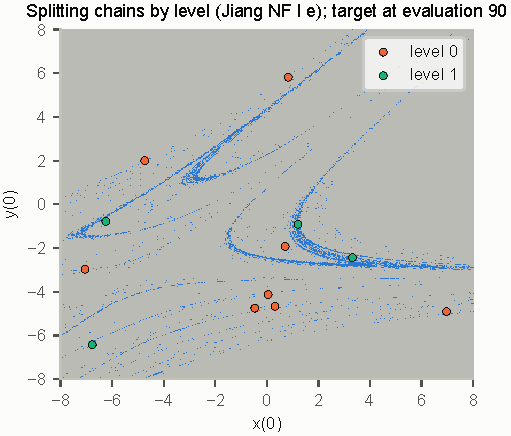
\includegraphics[width=\columnwidth]{figures/fig38_sus_chains.pdf}
\caption{Splitting chains on the basin map of the Jiang map NF~I~e (gray: escape; blue: basin of the chaotic attractor): seeds of levels 0 (open circles) and 1 (triangles). Already at the second level, the chains sit on thin ``tongues'' of the basin, since the escape step is larger near their edges; the target is found after 90 integrations. Seeds that coincide are drawn once.}
\label{fig:suschains}
\end{figure}

\subsection{Active learning of basin boundaries}\label{sec:al}

The active-learning arm stores all evaluated points with their labels; escaping trajectories form a separate class. On these data, a $k$-nearest-neighbor classifier ($k=10$, weights inversely proportional to distance) is trained in normalized coordinates of $B$. From a pool of 2000 candidates, the points with the largest entropy of the predicted class probabilities are selected for evaluation (uncertainty sampling\cite{Settles2012}). Half of the pool consists of Gaussian perturbations of ``boundary'' points of the sample, i.e., points that have a point of another class among their $k$ neighbors, with a scale of half the distance to the nearest neighbor of another class. The other half consists of uniform points or points of a prior set (nullclines). The classifier is retrained when the sample grows by 10\%. Two implementation choices keep the cost of this arm bounded (Appendix~\ref{app:implementation}): neighbors are found by brute-force search (for $n\ge6$, or while the sample has at most 2000 points), which returns the same queries several times faster than a tree, and in the two-stage configuration the classifier is trained on the last $2\times10^4$ evaluated points only. While the data contain a single class, there are no boundaries, and the arm is idle.

\subsection{Portfolio and worst-case guarantee}\label{sec:portfolio}

In each round, the portfolio evaluates a batch of points from the splitting arm (10 points), from the active-learning arm (20 points if the data contain at least two classes), and uniform points. The number of uniform points is $\lceil\theta/(1-\theta)\cdot n_{\rm arm}\rceil$, where $n_{\rm arm}$ is the number of points from the arms and $\theta=0.2$ is the uniform share. Points within a batch are shuffled so that no arm is favored in the accounting of the first-hit time. The reference sample is shared by both arms. An arm is called \emph{autonomous} if the choice of its points depends only on the results of its own evaluations. The uniform arm and the splitting arm are autonomous; the active-learning arm uses all data. The uniform share plays the role of the defensive component of mixture importance sampling,\cite{Hesterberg1995} and combining strategies with different failure modes follows the idea of algorithm portfolios, which reduce the risk of heavy-tailed run times.\cite{Huberman1997,GomesSelman2001}

\begin{proposition}\label{prop:portfolio}
Let $c$ be the maximum batch size, $\omega_j$ the guaranteed share of arm $j$ in each round, and $N_{1-\delta}(j)$ the cost of arm $j$ run on its own. Then
\begin{equation}
\begin{split}
N_{1-\delta}(\text{portfolio})\le\min\biggl\{&\frac{N^0_{1-\delta}+c}{\theta},\\
&\min_{j\ \text{autonomous}}\frac{N_{1-\delta}(j)+c}{\omega_j}\biggr\}.
\end{split}
\label{eq:portfolio}
\end{equation}
\end{proposition}
\textit{Proof.} After $N$ evaluations of the portfolio, an autonomous arm $j$ has performed at least $\omega_jN-c$ evaluations of its own. By autonomy, the sequence of its points is distributed as in a stand-alone run with the same generator. Therefore, $\Pr[\tau>N]\le\Pr[\tau_j>\omega_jN-c]\le\delta$ whenever $\omega_jN-c\ge N_{1-\delta}(j)$. For the uniform arm, $N_{1-\delta}(j)=N^0_{1-\delta}$ and $\omega_j=\theta$. \hfill$\blacksquare$

The proposition is an elementary property of a defensive mixture, and its value is in the construction it justifies. Its consequences are as follows. First, in the number of integrations, the portfolio is at most $1/\theta=5$ times costlier than uniform sampling, up to the additive term $c/\theta$: $G\ge\theta N^0/(N^0+c)$, which for $c=38$ and $N^0\approx200$ is 0.17 rather than 0.2. A single adaptive method has no such bound: splitting alone, and novelty search driven by asymptotic features (Appendix~\ref{app:ablation}), fail to find the target within the budget in some runs. Second, the scaling exponent of the portfolio is no larger than that of the best autonomous arm: a constant factor $1/\omega_j$ is lost, but not the order. In our implementation, the share of the splitting arm is $\omega\approx0.26$ when the active-learning arm is active and $\omega\approx0.77$ without it. Two qualifications apply. The bound holds in integrations, not in integrator steps or wall time: the arms select long transients, so a point of the portfolio may cost more steps than a uniform point (Sec.~\ref{sec:cost}). Autonomy of the splitting arm is exact with full integration; with two-stage evaluation and templates that grow during the search (Sec.~\ref{sec:twostage}), the coordinate of its points depends weakly on what the other arms have found, so the inheritance of its exponent is then approximate, and the bound through the uniform arm requires that stage~1 never stops a target trajectory, which is verified in Sec.~\ref{sec:cost}.

\subsection{Cost model and channel diagnostics}\label{sec:costmodel}

Splitting with selection fraction $p_0$ builds nested sets $S_l=\{\xi\ge\xi_l\}$ with $\mu(S_{l+1}\mid S_l)\approx p_0$; one level costs $n_0(1-p_0)$ evaluations. Denote by $\pi_l=\mu(W^*\mid S_l)$ the fraction of the target in the $l$th set and by $e_l=\pi_{l+1}/\pi_l\in[0,1/p_0]$ the enrichment at level $l$; $e_l<1$ means that the coordinate is deceptive at that level. The target becomes frequent when $\prod_{l<K}e_l\approx1/p$, and the cost is $N\approx n_0+n_0(1-p_0)K+O(1/\pi_K)$.

\begin{proposition}[cost model]\label{prop:cost}
Assume that the chains sample the conditional distribution on each $S_l$ exactly, that the number of levels is unbounded, and that the final stage samples $S_K$ independently. (i)~If the coordinate is ideal, $e_l=1/p_0$, then $K=\lceil\ln(1/p)/\ln(1/p_0)\rceil$ and $N=O(n_0\ln(1/p))$, i.e., $s=0$. (ii)~If the enrichment is constant, $e_l=p_0^{-\zeta}$ with $0<\zeta\le1$, then $K\approx\ln(1/p)/(\zeta\ln(1/p_0))$, and the cost is still logarithmic. (iii)~If the coordinate is informative only down to a depth $K^*$ ($e_l=1$ for $l>K^*$), then $N\approx n_0+n_0(1-p_0)K^*+1/\pi_{K^*+1}$: the scaling exponent returns to $s=1$, with a constant-factor gain $\prod_{l\le K^*}e_l$. (iv)~If the coordinate is deceptive, $e_l<1$, the same count gives a constant factor below 1, i.e., a loss.
\end{proposition}

Proposition~\ref{prop:cost} follows from counting levels. It is a model of the mechanism rather than a statement about the implementation: the implementation restarts after ten levels, so the logarithmic regime is available only while $p\ge p_0^{10\zeta}$; the states of a chain are correlated samples, which is why a coordinate with zero informative depth gives $G<1$ rather than $G=1$ (family D1, Sec.~\ref{sec:scaling_p}); and the exponent $s\approx0.45$ observed on D2 over $p=10^{-2}$--$10^{-5}$ (Sec.~\ref{sec:scaling_p}) is a crossover between the logarithmic regime at $p\gtrsim10^{-4}$ and the discretization limit below it, not an asymptotic law. Its content lies in the classification: an order-of-growth gain requires a coordinate that is informative on all scales, a finite informative depth yields a constant-factor gain, and a deceptive coordinate yields a loss. The transient duration diverges at a basin boundary, where the trajectory follows the stable manifold of the edge state. If the target basin is surrounded by such a boundary and the sets $S_l$ are nested all the way down to it, the enrichment persists on all scales (the case of D2). If the boundary of the target does not stand out against other boundaries, or if the duration saturates, only the near zone is informative. Saturation occurs, for example, for the discrete escape times of maps and for escape by slow drift.

\textbf{Diagnostics from the uniform sample.} The enrichment $e_l$ is not observable before the target is detected, but on a benchmark system with a known target, it can be estimated from a uniform sample. The decisive quantity is not the fraction of target points in the upper set $S_q$ (the fraction $q$ of points with the largest $\xi$) but spatial convergence toward the target. Let $d(q)$ be the median distance (in units of $L$) from the nontarget points of $S_q$ to the nearest target point of the sample. Splitting gains if $d(q)$ decreases as $q$ decreases: the chains move by a local random walk and need a connected ``path'' of ever longer transients leading to the basin. If $d(q)$ does not decrease, the long trajectories are scattered over the region, and there is no gain even if the fraction of the target in $S_q$ grows (Appendix~\ref{app:diagnostics}).

\textbf{Discretization limit.} The coordinate is built from a trajectory with step $\Delta t$, so escape times shorter than one step are indistinguishable. In D2, the escape time for $|w_0|\gg\rho$ equals $\rho^2/(2\kappa|w_0|^2)$, and the coordinate is informative only for $|w_0|\lesssim\rho/\sqrt{2\kappa\Delta t}$. The size of this zone relative to the region sets the limit of the gain at small $p$ and small $m$ (Sec.~\ref{sec:scaling_p}, Appendix~\ref{app:smallp}).

\subsection{Two-stage evaluation}\label{sec:twostage}

Most of the integration budget goes to trajectories that settle early onto a known regime yet are integrated over the full horizon, which the protocol requires only for target candidates (Sec.~\ref{sec:protocol}). We therefore evaluate every initial condition in two stages, for all strategies including uniform sampling. Stage~1 integrates the transient segment up to the end of the early window, $\min(n_{\rm tr},n_{\rm obs})$ steps, where $n_{\rm tr}$ and $n_{\rm obs}$ are the numbers of steps of the transient segment and of the observation window, followed by a short observation window of $n_{\rm obs}/4$ steps. The trajectory stops after stage~1 if, on this window, it is identified with confidence as a known nontarget regime: an equilibrium (converged, or decaying with an amplitude below $0.02L$), or a known cycle or chaotic attractor with a $z$ score below half the identification tolerance. Escaping trajectories are final anyway. All other trajectories (target candidates and unknown or ambiguous ones) continue from the end of the early window to the full horizon. Since the main trajectory and the early window are the same, their fingerprints coincide bit for bit with those of a single full integration, and the target is always confirmed by the full protocol. A stopped trajectory keeps its label; only its $\xi$ is computed on the shorter window.

For continued trajectories, stage~1 costs extra steps, because a quarter of the observation window is integrated twice. A rule based on step counts therefore keeps the two-stage mode only while it pays. After the first 200 evaluations, the mode stays on as long as the steps saved over the last ten batches exceed the extra steps; otherwise, only every tenth batch is evaluated in two stages, as a probe. The rule uses step counts rather than time, so runs remain reproducible. On uniform samples from eight problems, the two-stage labels and the fingerprints of all continued and escaping trajectories coincided with those of full integration bit for bit, and no target hit was lost (Sec.~\ref{sec:cost}).

\section{Results}\label{sec:results}

\subsection{Measurement protocol}\label{sec:measure}

For each ``system $\times$ strategy'' pair, we performed $R$ independent runs with fixed generator seeds: $R=100$ for levels A and B, the synthetic families, and the ablation; $R=50$ for the hyperparameter, horizon, bisection, and enlarged-region tests; and $R=10$--$100$ for the coupled systems. A run stopped at the first hit of the target or when the budget was exhausted. Common random numbers were used: the first 50 points of all strategies coincide with the first 50 points of uniform sampling, so differences arise only after the initial sample. $N_{0.9}$ is the 0.9 quantile of the first-hit time (infinity if fewer than 90\% of the runs find the target). Confidence intervals are 95\% bootstrap intervals over runs\cite{EfronTibshirani1994} (2000 resamples). The exponent $s$ is the slope of the regression of $\ln N_{0.9}$ on $\ln(1/p)$. Uniform sampling for the coupled systems and the enlarged regions was run on a GPU with a kernel that reproduces the CPU trajectories and fingerprints bit for bit. Unless stated otherwise, gains refer to the number of integrations with full integration. In the cost measurements (Sec.~\ref{sec:cost}), we also record integrator steps (a step of the observation window counts twice, because the companion trajectory for the Lyapunov exponent is integrated alongside) and wall time, measured after an untimed warm-up that compiles the kernels; steps and time up to the first hit are counted in proportion to the position of the hit within its batch. We compare uniform sampling, Zelinka's DE, splitting by $\xi$ from Eq.~\eqref{eq:xi}, active learning with 20\% uniform points, the portfolio, and the portfolio with nullclines (channel C). The final configuration of the portfolio (Sec.~\ref{sec:cost}) adds two-stage evaluation and the capped boundary arm; on runs shorter than $2\times10^4$ evaluations, the cap changes nothing. The library and the experiment scripts were written with the assistance of the AI coding assistant Claude (Anthropic; used through Claude Code in 2026, most recent model Claude Fable 5.1) to speed up the implementation of the author's specifications; all numerical results were produced by this code from fixed seeds, and the code was verified by the bit-exactness tests between the CPU and GPU kernels, by the independent integrators of Sec.~\ref{sec:protocol}, and by the agreement of its labels with Attractors.jl (Sec.~\ref{sec:cost}).

\subsection{Rare targets of levels A and B}\label{sec:rare_ab}

The results are summarized in Table~\ref{tab:gains} and Fig.~\ref{fig:pn}. The portfolio outperforms uniform sampling with statistical significance (the lower bound of the interval exceeds 1) on Chua~II (7.4 times), SE11 (3.1), and LE1 (6.2); with nullcline sampling, it also gains on Chua~I (4.4 times). On LE1, the best single arm is splitting (8.3 times), whereas active learning loses to uniform sampling (0.48): the long ``continuum of equilibria/escape'' boundary attracts the queries, and the target adjoins it only along a small part. The portfolio limits this degradation. On three problems, the portfolio gains little or nothing: the Jafari cycle, the Jafari chaos, and the Huynh map. These are predicted failures (Sec.~\ref{sec:failures}), and the portfolio stays within the guarantee of Proposition~\ref{prop:portfolio} ($G\ge\varepsilon=0.2$): 0.43, 0.42, and 1.40. Zelinka's DE, which is told the size of the target, is nowhere significantly better than uniform sampling; on the Jafari chaos and cycle, it loses by factors of 4.3 and 3.4. On the Jiang maps ($p\approx0.03$--$0.07$), all strategies are close to uniform sampling: at such $p$, the target is often found within the initial sample, and adaptation has nothing to work with. The contributions of the arms (ablation), the comparison with bisection toward basin boundaries, and the robustness to hyperparameters and to the integration horizon are given in Appendix~\ref{app:ablation}; no hyperparameter variant brings the gain below 1, and scaling both integration windows by 0.5 or 2 keeps the gains within 20\% of the base values.

\begin{table*}
\caption{Gain factors $G_{0.9}=N^0_{0.9}/N_{0.9}$ with 95\% bootstrap intervals ($R=100$). Bold: values whose lower interval bound exceeds 1.}
\label{tab:gains}
\footnotesize
\setlength{\tabcolsep}{4pt}
\begin{ruledtabular}
\begin{tabular}{lrrrrrrr}
System & $p$ & $N^0_{0.9}$ & \shortstack{Zelinka's\\DE} & Splitting & \shortstack{Active learning\\+ 20\% uniform} & Portfolio & \shortstack{Portfolio\\+ nullclines} \\
\hline
Chua I & 0.035 & 66 & 0.60 \ci{0.43}{0.99} & 1.20 \ci{0.92}{1.77} & 1.23 \ci{0.95}{1.74} & 1.24 \ci{0.94}{1.77} & \textbf{4.42} \ci{3.27}{6.47} \\
Chua II & 0.0027 & 818 & 0.84 \ci{0.67}{1.32} & \textbf{5.05} \ci{4.13}{7.07} & \textbf{3.16} \ci{2.58}{4.90} & \textbf{7.36} \ci{6.09}{10.2} & \textbf{7.64} \ci{5.98}{11.8} \\
SE11 & 0.0079 & 317 & 0.95 \ci{0.72}{1.07} & \textbf{2.53} \ci{1.95}{2.86} & \textbf{3.62} \ci{2.63}{4.16} & \textbf{3.10} \ci{2.46}{3.70} & \textbf{3.56} \ci{2.71}{4.31} \\
LE1 & 0.0016 & 1617 & 1.31 \ci{0.94}{2.08} & \textbf{8.29} \ci{6.35}{12.3} & 0.48 \ci{0.32}{1.49} & \textbf{6.24} \ci{3.76}{10.0} & \textbf{4.62} \ci{3.03}{10.7} \\
Jafari 2026, cycle & 0.009 & 219 & 0.29 \ci{0.19}{0.50} & 0.29 \ci{0.19}{0.53} & 0.88 \ci{0.66}{1.41} & 0.43 \ci{0.29}{0.78} & 0.32 \ci{0.25}{0.50} \\
Huynh 2019 & 0.0091 & 221 & 0.45 \ci{0.34}{0.85} & 1.36 \ci{0.79}{2.42} & 0.82 \ci{0.57}{1.72} & \textbf{1.40} \ci{1.16}{2.54} & --- \\
Jafari 2026, chaos & $(2$--$4)\times10^{-4}$ & 5265 & 0.23 \ci{0.16}{0.28} & 0.22 \ci{0.15}{0.28} & 1.08 \ci{0.57}{1.40} & 0.42 \ci{0.29}{0.58} & 0.27 \ci{0.16}{0.32} \\
\hline
Jiang NF I e/f/g & 0.028--0.039 & 109/86/71 & 0.83/0.90/1.00 & 1.52/1.23/1.08 & 1.02/1.51/1.15 & 1.46/1.49/1.23 & --- \\
Jiang SF I a/b & 0.065 & 36/33 & 0.75/0.92 & 1.00/1.00 & 1.00/1.00 & 1.00/1.00 & --- \\
\end{tabular}
\end{ruledtabular}
\end{table*}

\begin{figure*}
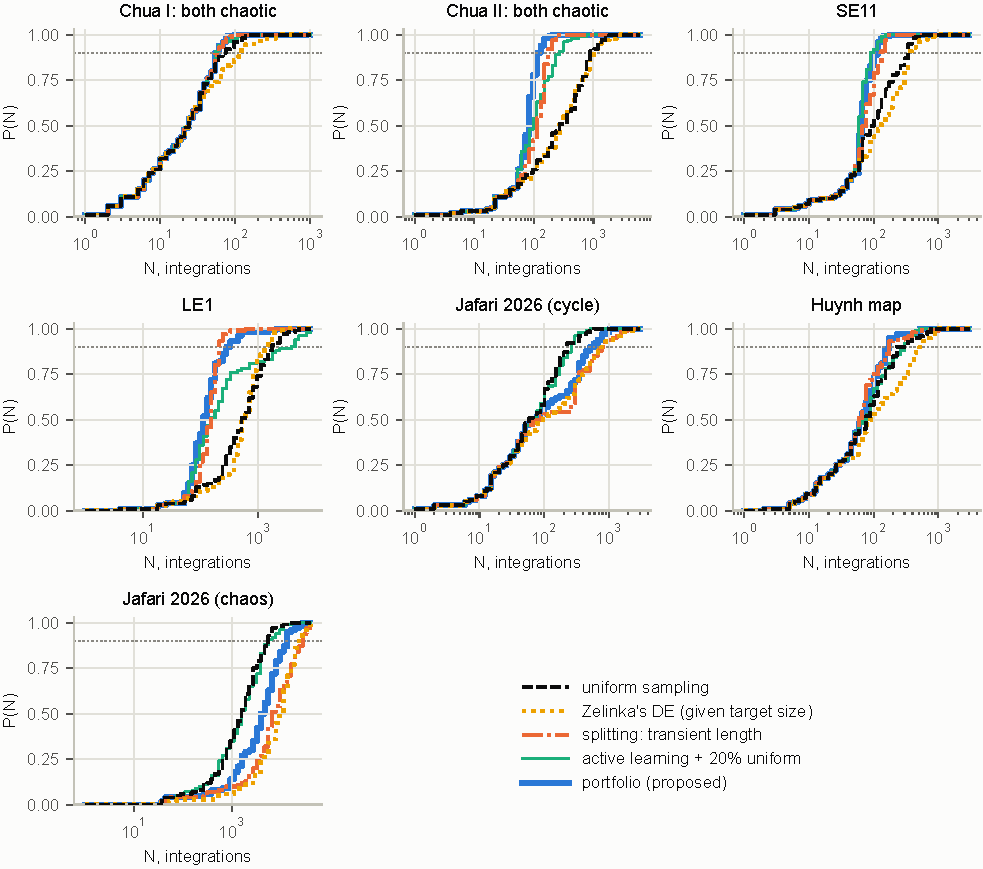
\includegraphics[width=\textwidth]{figures/fig21_pn_levelAB.pdf}
\caption{Detection probability $P(N)$ as a function of the number of integrations for rare targets of levels A and B ($R=100$ runs). The dotted line is the 0.9 level. On Chua~II, SE11, and LE1, the portfolio curve (thick blue) lies to the left of uniform sampling (gray) over the whole range; on the Jafari cycle and chaos, it lies to the right, but within the guaranteed factor $1/\varepsilon$.}
\label{fig:pn}
\end{figure*}

\subsection{Scaling with basin measure and dimension}\label{sec:scaling_p}

On family D2 ($n=6$), the gain grows as $p$ decreases from $10^{-2}$ to $10^{-5}$ (Table~\ref{tab:scaling}, Fig.~\ref{fig:scalp}). The scaling exponent of the portfolio is $s=0.45$ [0.42, 0.51], and that of splitting by $\xi$ is $0.41$ [0.37, 0.46], against $0.99$ [0.93, 1.04] for active learning and $0.95$ [0.90, 1.03] for uniform sampling (theoretical value 1). On a problem with a graded signal, the method thus gains in order: at $p=10^{-5}$, the gain is 93-fold for splitting and 72-fold for the portfolio. On family D1, where there is no signal outside the thin rim of the ball, all strategies have $s$ from 0.67 to 0.98; splitting does not help ($G=0.49$--$0.70$), and active learning gives a factor of 1.1--3.5 that grows as $p$ decreases, because escapes inside the ball serve as boundary markers. This is the prediction of Proposition~\ref{prop:cost} for a coordinate with zero informative depth.

Below $p=10^{-5}$, the gain on D2 breaks down: at $p=10^{-6}$, within $2\times10^5$ integrations, the portfolio finds the target in 35\% of runs against 18\% for uniform sampling, and at $10^{-7}$, within $10^6$ integrations, in 16\% against 9.5\%. The breakdown is the discretization limit of Sec.~\ref{sec:costmodel}: the coordinate is informative only in the zone $|w_0|\lesssim\rho/\sqrt{2\kappa\Delta t}$, which occupies 2.3\% of the region at $p=10^{-5}$, 0.23\% at $10^{-6}$, and 0.023\% at $10^{-7}$, so an initial sample of 50 points contains an informative point with probability 0.68, 0.11, and 0.011. Reducing the integration step restores the gain: fourfold at $p=10^{-6}$ gives $G=450$ for the portfolio and 530 for splitting, and sixteenfold at $p=10^{-7}$ gives 1200 and 1400, with all runs successful (Appendix~\ref{app:smallp}). The limit is set by the time resolution of the reaction coordinate rather than by splitting. The same limit explains the dependence on dimension at fixed $p=10^{-4}$ (Appendix~\ref{app:smallp}): the portfolio gains 17 times at $n=6$, 42 at $n=8$, 53 at $n=10$, 61 at $n=12$, and 45 at $n=14$, but nothing at $n=4$, where the basin in the additional coordinate has width $\rho=6.6\times10^{-4}$ and the coordinate is flat on 99.5\% of the region.

\begin{table}
\caption{Family D2 ($n=6$): cost of uniform sampling $N^0_{0.9}$ (in parentheses, the theoretical value $\ln10/p$) and the costs and gains of splitting and of the portfolio ($R=100$). For $p\le10^{-6}$, the budget of the strategies ($2\times10^5$ at $p=10^{-6}$ and $10^6$ at $p=10^{-7}$) is smaller than $N^0_{0.9}$, and the fraction of runs that found the target within it is given, with that of uniform sampling in brackets.}
\label{tab:scaling}
\begin{ruledtabular}
\begin{tabular}{rrrr}
$p$ & Uniform & Splitting & Portfolio \\
\hline
$10^{-2}$ & 277 (230) & 121 (2.3$\times$) & 122 (2.3$\times$) \\
$10^{-3}$ & 1932 (2303) & 262 (7.4$\times$) & 329 (5.9$\times$) \\
$10^{-4}$ & 17\,416 (23\,026) & 714 (24$\times$) & 1026 (17$\times$) \\
$10^{-5}$ & 189\,765 (230\,259) & 2039 (93$\times$) & 2634 (72$\times$) \\
$10^{-6}$ & $2.19\times10^{6}$ ($2.30\times10^{6}$) & 24\% [18\%] & 35\% [18\%] \\
$10^{-7}$ & $2.14\times10^{7}$ ($2.30\times10^{7}$) & 9\% [9.5\%] & 16\% [9.5\%] \\
\end{tabular}
\end{ruledtabular}
\end{table}

\begin{figure*}
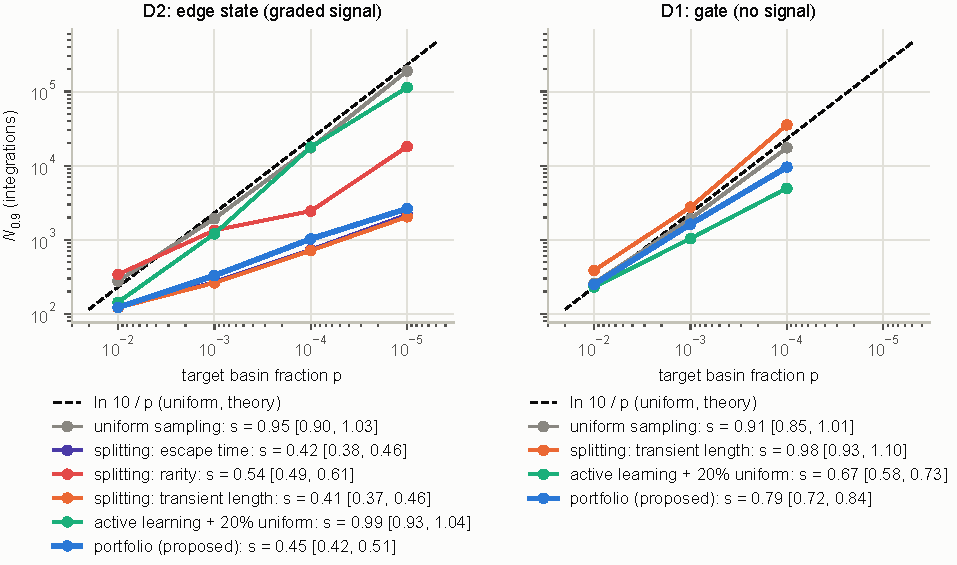
\includegraphics[width=\textwidth]{figures/fig23_scaling_p.pdf}
\caption{Detection cost $N_{0.9}$ versus basin measure $p$ ($n=6$, $R=100$); the legends give the scaling exponents $s$, defined by $N_{0.9}\propto p^{-s}$, with 95\% intervals. Left: family D2 with a graded signal; the splitting arms and the portfolio have $s\approx0.4$--$0.45$. Right: family D1 without a signal; all strategies have $s\approx0.7$--$1$. Dashed line: $\ln10/p$.}
\label{fig:scalp}
\end{figure*}

\subsection{Coupled systems: rare hidden targets and a new attractor}\label{sec:coupled}

\textbf{Coupled copies of SE11.} A real system with a rare hidden target is obtained by coupling several copies of a system with a hidden attractor. We take $k$ copies of SE11 with mean-field coupling along $y$:
\begin{equation}
\dot{\bm x}_u=\bm F(\bm x_u)+\epsilon\,\bigl(\bar y-y_u\bigr)\,\bm e_y,\qquad u=1,\dots,k,
\label{eq:coupled}
\end{equation}
where $\bar y=k^{-1}\sum_{v}y_v$ and $\epsilon=0.01$, in the region $B^k$. The only equilibrium is the synchronous equilibrium of SE11, which is stable, so the regime ``all copies on the hidden attractor'' is hidden. Its basin measure is $5.5\times10^{-5}$ for $k=2$ ($n=6$) and $3.5\times10^{-7}$ for $k=3$ ($n=9$), close to $p_1^k$ for independent copies ($p_1=0.0079$). Here the portfolio gains by orders of magnitude (Table~\ref{tab:coupled}): 65 \ci{42}{87} at $n=6$ and 1400 \ci{900}{2400} at $n=9$, where it needs about $5\times10^3$ integrations instead of $7.6\times10^6$; all runs found the target. The transient duration is set by the copies that have not yet settled, so successive levels of splitting fix the copies one after another, and the cost grows roughly geometrically in $k$ with a ratio far smaller than $1/p_1$. Without coupling, the gains are the same (1600 at $n=9$), and with four uncoupled copies ($n=12$, $p=p_1^4=3.9\times10^{-9}$), the portfolio finds the target in $N_{0.9}=4.7\times10^4$ integrations, a gain of $1.3\times10^4$ relative to the exact uniform cost $\ln10/p$. Bisection toward basin boundaries does not scale on these systems: within budgets of $8/p$ at $n=6$ and $2\times10^5$ at $n=9$, it finds the target in 66\% and 32\% of runs. The coupling is weak, and the problem is close to a product of independent ones; if the attractors of a single copy are known, product initial conditions reach such a target directly, so the coupled copies test the mechanism of the gain rather than replace that shortcut.

\begin{table*}
\caption{Coupled copies of SE11, Eq.~\eqref{eq:coupled}: basin measure of the regime ``all copies on the hidden attractor,'' cost of uniform sampling, and gains $G_{0.9}$ with 95\% bootstrap intervals ($R=100$ for $n=3$ and for $n=9$ with coupling; $R=50$ otherwise). For $n=12$, $N^0_{0.9}=\ln10/p_1^4$ is the exact geometric value. Bold: values whose lower interval bound exceeds 1.}
\label{tab:coupled}
\footnotesize
\setlength{\tabcolsep}{3pt}
\begin{ruledtabular}
\begin{tabular}{rrrrrr}
$n$ & $\epsilon$ & $p$ & $N^0_{0.9}$ & Splitting & Portfolio \\
\hline
3 & --- & $7.7\times10^{-3}$ & 317 & \textbf{2.53} \ci{1.95}{2.86} & \textbf{3.10} \ci{2.46}{3.70} \\
6 & 0.01 & $5.5\times10^{-5}$ & $3.8\times10^{4}$ & \textbf{44.0} \ci{27.0}{65.6} & \textbf{64.9} \ci{41.7}{86.6} \\
9 & 0.01 & $3.5\times10^{-7}$ & $7.6\times10^{6}$ & \textbf{682} \ci{448}{989} & \textbf{1435} \ci{896}{2372} \\
9 & 0 & $4.9\times10^{-7}$ & $5.3\times10^{6}$ & \textbf{598} \ci{325}{1000} & \textbf{1574} \ci{771}{2299} \\
12 & 0 & $3.9\times10^{-9}$ & $5.9\times10^{8}$ & \textbf{4881} \ci{3860}{6354} & \textbf{12\,681} \ci{9827}{18\,098} \\
\end{tabular}
\end{ruledtabular}
\end{table*}

\textbf{Two coupled Chua circuits.} The trajectories of SE11 mostly escape, so a uniform sample is cheap (Sec.~\ref{sec:cost}). A system in which all trajectories are bounded is obtained from two Chua~II circuits with mutual coupling $\epsilon(\bar x-x_u)$ in the first equation, $\epsilon=0.1$. The nine equilibria (products of the equilibria of the single circuit) are found by Newton's method; the regimes of the coupled system are enumerated by the identification protocol on a uniform sample of $5\times10^4$ points, with the products of the attractors and stable equilibria of the single circuit as initial templates. The synchronized cycle LC takes 98\% of the region. The rare hidden family consists of the regimes in which one circuit is on a hidden chaotic attractor and the other is at a stable equilibrium (and, at weaker coupling, both on hidden attractors); its total basin measure is $2.3\times10^{-5}$, and no trajectory from the $10^{-3}L$ and $10^{-2}L$ neighborhoods of the equilibria reaches it. On this target, with two-stage evaluation, the portfolio needs $N_{0.9}=1900$ integrations against $1.05\times10^5$ for uniform sampling ($R=20$, all runs successful), a gain of 55 in integrations and 64 in wall time (Table~\ref{tab:cost}). Three uncoupled copies of Chua~II give the extreme case: the regime ``every copy on one of its two hidden attractors'' has $p=(p_a+p_b)^3=1.9\times10^{-8}$ exactly, beyond uniform sampling ($\ln10/p=1.2\times10^8$ integrations, about four days of computing); the final configuration of the portfolio finds it in 9 of 10 runs within $4\times10^5$ integrations, with a median of $8.6\times10^4$ and $N_{0.9}=3.2\times10^5$, a gain of 370 in integrations and 150 in time.

\textbf{A hidden attractor born by the coupling.} The same enumeration revealed a regime that the single circuit does not have (Fig.~\ref{fig:newattr}): one circuit stays on the large cycle LC, and the other hops chaotically between the regions of the two hidden attractors HA$_a$ and HA$_b$, which in the single circuit at these parameters never merge.\cite{Stankevich2017} The regime passes the verification protocol (lifetime over $2\times10^3$ time units, the same template at $dt/2$, $\lambda=0.10$), and it is hidden: none of 3624 trajectories started in the $10^{-3}L$ and $10^{-2}L$ neighborhoods of the nine equilibria and along their unstable directions reaches it ($h_\varepsilon=0.18$ at $10^{-1}L$, as for Chua~I). Continuation in the coupling shows how it arises: for $\epsilon<0.045$, the second circuit oscillates periodically near one of its stable equilibria (four symmetric periodic regimes); at $\epsilon\approx0.045$, these branches merge into the chaotic hopping; $\lambda$ grows almost linearly to 0.35 at $\epsilon=0.46$, with periodic windows at $\epsilon=0.09$ and $0.47$; and at $\epsilon\approx0.5$, the two branches merge with the synchronized cycle. Coupled Chua circuits with hidden attractors have been studied for synchronization,\cite{Stankevich2017,Kuznetsov2023Chua} and we have not found this regime reported. It is hidden but not rare: its basin fraction is 0.6--1\% per symmetric branch at all $\epsilon$. Table~\ref{tab:newattr} compares how fast the search methods find it: the standard procedure never does, uniform sampling and the portfolio find it within a few hundred integrations, and if the attractors of the single circuit are known, the product initial condition ``LC $\times$ HA$_a$'' lands on it in one integration, because the regime continues that product state. The value of the method here is the enumeration with verification rather than speed.

\begin{figure*}
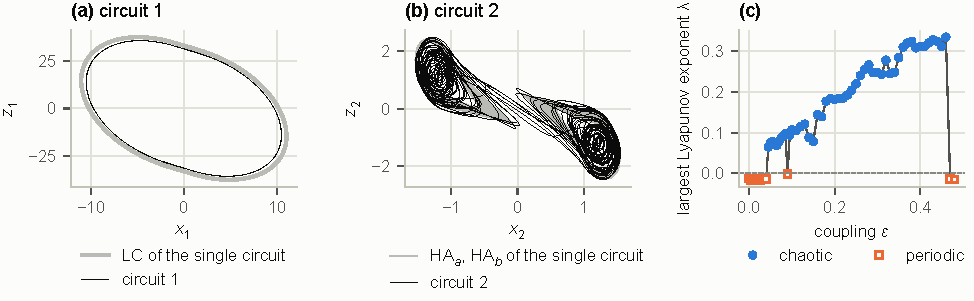
\includegraphics[width=\textwidth]{figures/fig31_new_attractor.pdf}
\caption{Hidden attractor of two coupled Chua~II circuits born by the coupling ($\epsilon=0.1$). (a) Circuit 1 in the projection $(x_1,z_1)$ against the cycle LC of the single circuit. (b) Circuit 2 in $(x_2,z_2)$ against the hidden attractors HA$_a$ and HA$_b$ of the single circuit (gray): the trajectory hops between their regions. (c) Largest Lyapunov exponent of the regime versus the coupling, from continuation in $\epsilon$: chaos is born at $\epsilon\approx0.045$ by merging of periodic branches and disappears at $\epsilon\approx0.5$.}
\label{fig:newattr}
\end{figure*}

\begin{table}
\caption{Finding the coupling-born attractor of Fig.~\ref{fig:newattr} (basin fraction 0.016 for the two symmetric branches): integrations to detection (0.9 quantile and median over $R=20$ runs) and wall time $T_{0.9}$ on one thread. The times of uniform sampling with two-stage evaluation and of the portfolio are measured; those of full integration and of recurrence-based stopping (Attractors.jl, Sec.~\ref{sec:cost}) are rescaled from the two-stage time by the measured ratio of costs per evaluation.}
\label{tab:newattr}
\footnotesize
\begin{ruledtabular}
\begin{tabular}{lrrr}
Method & $N_{0.9}$ & Median & $T_{0.9}$, s \\
\hline
From neighborhoods of the equilibria & never & --- & --- \\
Uniform sampling, full integration & 230 & 18 & 28 \\
Uniform sampling, two-stage evaluation & 230 & 18 & 17 \\
Uniform sampling, Attractors.jl & 230 & 18 & 6.4 \\
Portfolio (final configuration) & 81 & 18 & 8.1 \\
Product of single-circuit attractors & 1 & 1 & 0.07 \\
\end{tabular}
\end{ruledtabular}
\end{table}

\subsection{Cost in integrator steps and wall time}\label{sec:cost}

The number of integrations is a fair measure of cost only if all integrations cost about the same. They do not when trajectories escape: an escaping trajectory stops at the step of escape, and the method deliberately concentrates on long-lived trajectories. We therefore measured the cost of the final configuration in integrator steps and wall time (Table~\ref{tab:cost}, Fig.~\ref{fig:cost}). The final configuration is the three-arm portfolio with two-stage evaluation (Sec.~\ref{sec:twostage}), brute-force neighbor search, and the boundary arm trained on the last $2\times10^4$ points; for coupled systems, all products of the attractors of single units except the target are declared known. The reference is uniform sampling with the same two-stage evaluation. The gains are $G_N$ in integrations, $G_S$ in steps, and $G_T$ in time ($R=20$; three copies of Chua~II: $R=10$).

\begin{table*}
\caption{Cost of the final configuration of the portfolio relative to uniform sampling, both with two-stage evaluation ($R=20$; three copies of Chua~II: $R=10$, 9 successful runs): mean integrator steps per evaluation and gains in integrations ($G_N$), steps ($G_S$), and wall time ($G_T$, four threads per process). Bold: $G_T>1$. For uncoupled copies of Chua~II, uniform sampling is out of reach, and its cost is $\ln10/p$ evaluations at the measured cost per evaluation.}
\label{tab:cost}
\footnotesize
\begin{ruledtabular}
\begin{tabular}{lrrrrrrr}
Problem & $n$ & $p$ & \multicolumn{2}{c}{Steps per evaluation} & $G_N$ & $G_S$ & $G_T$ \\
 & & & Uniform & Portfolio & & & \\
\hline
%TABCOST-BEGIN
Chua I & 3 & $3.3\times10^{-2}$ & $2.6\times10^{4}$ & $4.6\times10^{4}$ & 1.0 & 0.27 & 0.25 \\
SE11 & 3 & $7.7\times10^{-3}$ & 1139 & 3681 & 4.1 & 0.92 & 0.84 \\
LE1 & 3 & $1.3\times10^{-3}$ & 334 & $1.1\times10^{4}$ & 2.1 & 0.052 & 0.085 \\
D2, $p=10^{-4}$ & 6 & $1.0\times10^{-4}$ & 14 & 1169 & 12 & 0.078 & 0.12 \\
D2, $p=10^{-5}$ & 6 & $1.0\times10^{-5}$ & 2 & 616 & 120 & 0.32 & \textbf{1.6} \\
2 coupled SE11 & 6 & $5.5\times10^{-5}$ & 117 & 3694 & 49 & 1.2 & \textbf{1.0} \\
3 coupled SE11 & 9 & $3.5\times10^{-7}$ & 45 & 3418 & 2600 & 30 & \textbf{22} \\
Chua II & 3 & $2.6\times10^{-3}$ & $8.7\times10^{4}$ & $9.7\times10^{4}$ & 6.3 & 5.3 & \textbf{3.8} \\
2 Chua II, $\epsilon=0.1$ & 6 & $2.3\times10^{-5}$ & $3.0\times10^{5}$ & $3.4\times10^{5}$ & 55 & 49 & \textbf{64} \\
2 Chua II, $\epsilon=0$ & 6 & $7.2\times10^{-6}$ & $1.7\times10^{5}$ & $1.9\times10^{5}$ & 200 & 160 & \textbf{130} \\
3 Chua II, $\epsilon=0$ & 9 & $1.9\times10^{-8}$ & $1.7\times10^{5}$ & $2.3\times10^{5}$ & 370 & 270 & \textbf{150} \\
%TABCOST-END
\end{tabular}
\end{ruledtabular}
\end{table*}

\begin{figure}
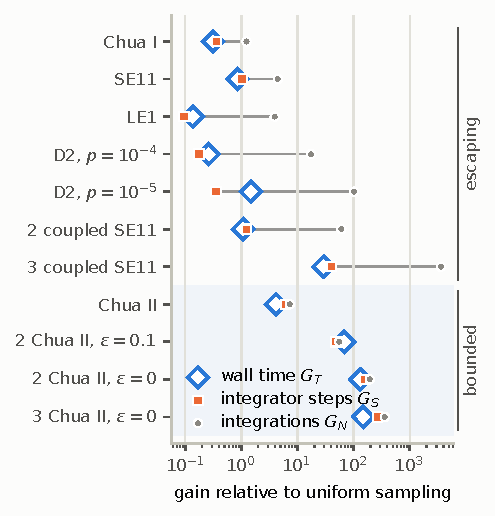
\includegraphics[width=\columnwidth]{figures/fig30_cost_gains.pdf}
\caption{Gain of the portfolio relative to uniform sampling in integrations ($G_N$), integrator steps ($G_S$), and wall time ($G_T$), both with two-stage evaluation. Above the dotted line: systems in which most trajectories escape quickly; below: systems with bounded trajectories. Dashed line: $G=1$.}
\label{fig:cost}
\end{figure}

The problems fall into two groups. In the systems where most trajectories escape quickly (Chua~I, SE11, LE1, D2, coupled SE11), the portfolio spends 2--300 times more steps per evaluation than uniform sampling, because it selects exactly the long transients that lead toward the target, whereas most uniform points escape within a few steps. The gain in integrations then shrinks in steps by a factor of 4--400, and the portfolio is slower than uniform sampling in time on Chua~I, SE11, LE1, and D2 at $p=10^{-4}$ (0.085--0.84). It gains in time only where the gain in integrations is large: 1.6 on D2 at $p=10^{-5}$ ($G_N=120$) and 22 on three coupled copies of SE11 ($G_N=2600$). In the systems with bounded trajectories (Chua~II and its coupled and uncoupled copies), every trajectory runs over the full horizon unless the two-stage evaluation stops it, the steps per evaluation of the portfolio and of uniform sampling are close, and the gain carries over to time: 3.8 on Chua~II, 64 on the coupled circuits, and 130--150 on the uncoupled copies. Two-stage evaluation makes both methods faster, uniform sampling more so: on Chua~II, 94\% of the uniform points and 91\% of the points of the portfolio stop at stage~1. Product references matter for coupled systems: they let stage~1 stop the trajectories that settle onto mixed states and give the boundary arm informative classes instead of ``unknown''; on three coupled copies of SE11, $N_{0.9}$ falls from 3500 to 2100 and $G_T$ grows from 4 to 12. The own computations of the arms take 1--8\% of the time on the Chua systems and 20--60\% on the cheap problems, mostly the nearest-neighbor queries of the boundary arm; brute-force search for $n\ge6$ reduces them by a factor of 1.6--2.6 ($G_T$ from 12 to 22 on three coupled copies of SE11), and the cap on the training sample removes their growth in long runs: on three uncoupled copies of Chua~II, it lowers the overhead from 51\% to 28\% and, by training the classifier on recent points only, also lowers the median cost from $1.4\times10^5$ to $8.6\times10^4$ integrations, so $G_T$ grows from 64 to 150. A wider batch, with two or four times more chains and boundary points to occupy more cores, does not pay: the number of evaluations grows by a factor of 1.5--3, whereas the time per evaluation decreases by about 10\% only.

\textbf{Comparison with recurrence-based evaluation.} The cost of one evaluation can be reduced further by stopping a trajectory as soon as it recurs in the cells of an already known attractor, as in Attractors.jl.\cite{DatserisWagemakers2022,Datseris2023Framework} For uniform sampling, the index of the first point in the target basin does not depend on how the trajectories are evaluated, so the time of uniform sampling with any evaluation scheme is $N^0_{0.9}$ times the mean cost of one evaluation, and the schemes can be compared on a common set of initial conditions. Table~\ref{tab:time} compares, on one thread, full integration, our two-stage evaluation, and \textsc{AttractorsViaRecurrences} (Attractors.jl 2.0, sparse grid of 100 cells per dimension, sampling interval 0.1, adaptive Tsit5 with tolerance $10^{-9}$ or fixed-step RK4 with our step), whose labels on the first 500 points coincide with ours and which recognizes the target states fed to it. On the bounded Chua systems with long transients, recurrence-based stopping is 2--3 times cheaper per evaluation than our two-stage evaluation, which still needs the early window and a quarter of the observation window for the fingerprint; on the escaping systems, our evaluation is 2--8 times cheaper, because escape is detected by the radius at once. Against uniform sampling with recurrence-based stopping, the time gain of the portfolio on the coupled Chua circuits falls from 27 to 10, and on Chua~II from 5 to 1.6; the gain in integrations is untouched. The search strategy and the evaluation back-end are independent choices: the portfolio needs only a regime label and a transient duration for each point, both of which the recurrence mapper provides, so combining the two would return the time gain to the gain in integrations.

\begin{table*}
\caption{Uniform sampling with three evaluation schemes against the portfolio, on one thread ($R=20$): cost of one evaluation (ms), time to detection $T_{0.9}$ (s), and the time gain of the portfolio relative to uniform sampling with two-stage evaluation ($G_T$) and with recurrence-based stopping ($G_T^{\rm rec}$). For uniform sampling, $T_{0.9}=N^0_{0.9}$ times the cost of one evaluation; for the portfolio, the measured 0.9 quantile of the run time. Attractors.jl: the fastest of the tested settings (Tsit5). Bold: gains above 1.}
\label{tab:time}
\footnotesize
\setlength{\tabcolsep}{3pt}
\begin{ruledtabular}
\begin{tabular}{lrrrrrrrrrrrr}
Problem & $p$ & $N^0_{0.9}$ & \multicolumn{3}{c}{Cost per evaluation, ms} & \multicolumn{3}{c}{$T_{0.9}$ of uniform sampling, s} & \multicolumn{2}{c}{Portfolio} & $G_T$ & $G_T^{\rm rec}$ \\
 & & & full & two-stage & Attractors.jl & full & two-stage & Attractors.jl & $N_{0.9}$ & $T_{0.9}$, s & & \\
\hline
%TABTIME-BEGIN
Chua II & $2.6\times10^{-3}$ & 710 & 26.7 & 6.07 & 1.95 & 19 & 4.3 & 1.4 & 113 & 0.87 & \textbf{5.0} & \textbf{1.6} \\
2 Chua II, $\epsilon=0.1$ & $2.3\times10^{-5}$ & 104980 & 72.8 & 44.8 & 16.4 & 7.6e3 & 4.7e3 & 1.7e3 & 1899 & 172 & \textbf{27.3} & \textbf{10.0} \\
SE11 & $7.7\times10^{-3}$ & 294 & 0.131 & 0.0562 & 0.131 & 0.038 & 0.016 & 0.038 & 71 & 0.028 & 0.6 & \textbf{1.4} \\
LE1 & $1.3\times10^{-3}$ & 858 & 0.021 & 0.0108 & 0.0819 & 0.018 & 0.0093 & 0.07 & 413 & 0.58 & 0.016 & 0.12 \\
%TABTIME-END
\end{tabular}
\end{ruledtabular}
\end{table*}

\subsection{Failures and limits}\label{sec:failures}

All failures are kept in the paper: they delineate the domain of applicability of the method.
\begin{enumerate}
\item \textbf{Deceptive coordinate (Jafari 2026 chaos).} Almost all trajectories escape to infinity by slow drift, and the longest escapes lie in the region of slow drift rather than near the attractor. Splitting finds the target 4.5 times more slowly than uniform sampling ($G=0.22$); the portfolio stays within the guarantee (0.42).
\item \textbf{Deceptive transients in an enlarged region.} Enlarging the region of initial conditions $k$ times about its center does not make the hidden attractors of the benchmark rare: the basins extend far beyond the natural region, and $p$ falls by one or two orders of magnitude at most instead of $k^3$ (Appendix~\ref{app:enlarged}). On SE11, LE1, and Chua~I, the gain grows as $p$ falls (to 24, 16, and 6.3), but on Chua~II at $k=4$, the longest transients belong to trajectories returning from far away, splitting alone loses by a factor of 7, and the portfolio stays within the guarantee (0.71).
\item \textbf{Islands among escaping trajectories without a gradient of duration.} For the Jafari cycle, the escape time is determined by slow drift, and for the Huynh map, the escape times are discrete. No arm gains on the Jafari cycle, and the portfolio gains only 1.4 times on the Huynh map.
\item \textbf{Long boundaries of known basins to which the target adjoins along a small part (LE1).} The active-learning arm has a median 3.7 times better than uniform sampling but a heavy tail: 17 of 100 runs get stuck near a remote part of the boundary, and two do not find the target within the budget. In the portfolio, this tail is bounded (median 109, maximum 1859 evaluations).
\item \textbf{Discretization limit at very small $p$} (D2, $p\le10^{-6}$; Sec.~\ref{sec:scaling_p}).
\item \textbf{Cheap nontarget trajectories.} Where most trajectories escape within a few steps, a gain of 2--120 in integrations is a draw or a loss in time (Sec.~\ref{sec:cost}).
\item \textbf{First-generation strategies.} Adaptive splitting driven by asymptotic novelty finds the target on Chua~II in only 55\% of runs, and MAP-Elites with a behavior descriptor gives a median 4 times better than uniform sampling but a heavy tail, $G=0.39$. Such tails are precisely what the uniform share of the portfolio removes.
\end{enumerate}
The channel diagnostic $d(q)$ of Sec.~\ref{sec:costmodel}, measured on uniform samples, separates the cases of gain and failure on all seven problems where it was tested (Appendix~\ref{app:diagnostics}).

\section{Discussion}\label{sec:discussion}

\textbf{What the rare-event formulation provides.} The formulation in terms of $P(N)$ and $N_{0.9}$ turns the statement ``the method finds a hidden attractor'' into a measurable and comparable one. It makes visible three things that the qualitative setting obscures. First, many classical examples are not hard search problems, because the basin of the hidden attractor occupies a noticeable part of the natural region (Table~\ref{tab:benchmark}). Second, on truly rare targets the heuristics, including evolutionary search with Zelinka's cost function,\cite{Zelinka2016} are no better than uniform sampling and sometimes worse (Table~\ref{tab:gains}). Uniform sampling is itself a strong reference: its cost $2.3/p$ is known in advance, does not depend on the geometry of the basin, and is within a factor of 2.6 of the best possible label-only algorithm (Sec.~\ref{sec:channels}). Third, rarity is a property of the chosen region rather than of the attractor: enlarging the region or moving the parameter toward the crisis of the attractor lowers the basin measure by one or two orders of magnitude at most (Appendix~\ref{app:enlarged}). A truly rare hidden target in a real system arises from a combination of several hidden regimes, as in coupled units (Sec.~\ref{sec:coupled}).

\textbf{When adaptive search gains.} A gain is possible only through the information carried by trajectories that missed the target (Sec.~\ref{sec:channels}), and the data confirm this. Channel B (transients) gives an order-of-growth gain if the transient duration grows on approach to the basin on all scales, as in D2 and, judging by the diagnostic $d(q)$, in basins surrounded by edge states (Chua~II, LE1, SE11); the enlarged regions of Appendix~\ref{app:enlarged} give effective exponents of 0.4--0.7 on SE11, LE1, and Chua~I, with the caveat that the geometry of the basin changes with the region. The most favorable case is a system of weakly coupled units with hidden attractors: the transient duration reports which units have not yet settled, splitting fixes them one after another, and the gain grows geometrically with the number of units. The order-of-growth gain is bounded in $p$ by the time resolution of the coordinate, so the time step is a parameter of the search, not only of the integration. Channel A (boundaries) works if the boundary of the known basins is short and the target forms a noticeable part of it. Channel C (prior sets) gives a gain when the heuristic is fortunate (nullclines for Chua~I) and costs nothing when it is not. The diagnostic $d(q)$ separates the cases of gain and failure on all seven problems where it was measured, but it requires a known target and therefore serves as a tool of analysis rather than prediction. The splitting arm is a multichain relative of the stagger-and-step method,\cite{SweetNusseYorke2001} which climbs the escape time of single trajectories to locate chaotic saddles. A single-chain climb on the same coordinate is as efficient as splitting or more where the signal is present, including the coupled copies and D2 down to $p=10^{-5}$, and, without a uniform share, falls below the bound of the portfolio where the coordinate is deceptive or uninformative (Appendix~\ref{app:ablation}). What matters for the gain is the coordinate, not the particular way of climbing it, and a stagger-and-step chain is a natural arm of the portfolio, under the same guarantee.

\textbf{When the gain is a gain in time.} Counting integrations treats a trajectory that escapes after a few steps and one that runs over the whole horizon as equal. The method selects the long ones by construction, so the count overstates its advantage wherever most trajectories escape quickly, and there the gain in integrations is a loss or a draw in time (Sec.~\ref{sec:cost}). Where trajectories are bounded, as in dissipative physical systems, a nontarget integration is as expensive as a target one, and the gain carries over to steps and to time. In time, the gain also depends on how fast the reference evaluates a trajectory: against uniform sampling with recurrence-based stopping, which needs no observation window, it is 2--3 times smaller than against uniform sampling with our two-stage evaluation. The two choices are independent: the portfolio needs from each trajectory only a regime label and a transient duration, which the recurrence mapper provides, so the next step is to combine them. The method thus pays in time when nontarget integrations are not cheap compared with the long transients it selects, or when the target is so rare that the gain in integrations exceeds the ratio of their costs.

\textbf{Why a portfolio is needed.} In the worst cases, single adaptive strategies lose to uniform sampling several times and produce heavy tails of the hit-time distribution (Sec.~\ref{sec:failures}). By Proposition~\ref{prop:portfolio}, the portfolio with a uniform share $\theta$ is guaranteed to cost no more than $1/\theta$ times uniform sampling in integrations and inherits the order of the best autonomous arm. On all failure problems, the portfolio stayed within these limits, whereas splitting alone fell well below them (Sec.~\ref{sec:failures}, Appendix~\ref{app:enlarged}), and the uniform share costs little on the favorable problems (Appendix~\ref{app:ablation}). Bisection toward basin boundaries\cite{NusseYorke1989,Skufca2006Edge} is a strong baseline on systems with smooth boundaries and costs nothing where there is no signal, but it loses where the signal is graded over many scales and does not scale to coupled units (Appendix~\ref{app:ablation}); as a fourth arm, it helps only where it is strong on its own.

\textbf{Relation to continuation and to compositional search.} The established way to find a rare attractor is to continue it from parameter values where it is easy to find, by path following or by global continuation.\cite{Brzeski2017,Datseris2023Framework,Datseris2026Global} This requires such a path; our method works at fixed parameters, which is the situation when a new system is explored or when the attractor exists only in a narrow parameter window. The two approaches are complementary: attractors found at neighboring parameter values are natural prior sets for channel C, and the portfolio can replace the uniform sample within each continuation step. For coupled units whose individual attractors are known, product initial conditions are another prior set, and in the coupled Chua circuits they reach both the rare family and the coupling-born attractor directly; the portfolio is for the case when the units' attractors are not known or the regime is not a product.

\textbf{Verification as part of the method.} Three episodes of this work (Appendix~\ref{app:verification}) show that without a verification protocol a comparison of search methods loses its meaning. False ``hidden attractors'' due to transient chaos are known;\cite{SprottMunmuangsaen2018Comment,Danca2016Transient} false ``absences'' due to the integration step are, according to our data, just as real. The same protocol, applied to enumerate the regimes of a new system, found the coupling-born attractor of the Chua circuits (Sec.~\ref{sec:newattr}). The hiddenness measure $h_\varepsilon$ complements the binary definition; what matters in practice is the scale at which neighborhoods of the equilibria cease to lead to the attractor, and for rare targets the number of starts must be large enough for a zero to be informative (Sec.~\ref{sec:coupled}).

\textbf{Limitations.} All conclusions about gains refer to the benchmark, the synthetic families, and the coupled copies. On other systems, a gain is not guaranteed; only the worst-case bound of Proposition~\ref{prop:portfolio} is, and only in integrations. For maps and for systems with escape by slow drift, the reaction coordinate may be uninformative or deceptive, and in a large region, slowly returning trajectories make it deceptive even for Chua~II. The discretization limit bounds the dynamic range of the coordinate by the time step. The gains of $10^3$--$10^4$ in integrations are obtained on weakly coupled or uncoupled copies, whose rare target is close to a product of the units' attractors; in that setting, declaring the product states of the units known improves the gain, and the numbers without this prior knowledge are reported alongside (Sec.~\ref{sec:cost}). The same formulation applies to trained models of dynamics, such as reservoir computers in closed loop,\cite{Pathak2017Chaos,LuHuntOtt2018} which may develop attractors absent from the training data;\cite{HaluszczynskiRath2019,HerteuxRath2020,Flynn2021,Kabayama2025PseudoLorenz} that application will be reported separately.

\section{Conclusions}\label{sec:conclusion}

The search for hidden attractors has been formulated as the detection of a rare event in the space of initial conditions, with the detection probability $P(N)$ and the cost $N_{0.9}$ relative to uniform sampling as the measures of quality. We have built a four-level benchmark with an identification and verification protocol and synthetic families with exactly known basin measure, and we have proposed a portfolio of multilevel splitting driven by transient duration, active learning of basin boundaries, and a uniform share, which in the worst case is at most $1/\varepsilon$ times costlier than uniform sampling and inherits the scaling exponent of the splitting arm.

On rare hidden attractors with $p\sim10^{-3}$--$10^{-2}$, the portfolio reduces the detection cost by factors of 3--7, with $R=100$ runs per problem. On a synthetic family with a graded signal, the cost grows as $p^{-0.45}$ instead of $p^{-1}$ down to $p=10^{-5}$; below this, the time resolution of the reaction coordinate limits the gain, and a proportionally smaller integration step restores it. On coupled copies of systems with hidden attractors, the gain in integrations reaches $10^3$--$10^4$. Counted in wall time, the gain depends on how expensive the nontarget trajectories are: where trajectories are bounded, as in the Chua circuits, it carries over, and on two coupled Chua circuits a rare hidden regime ($p=2\times10^{-5}$) is found 64 times faster than by uniform sampling with the same evaluation and 10 times faster than by uniform sampling with recurrence-based early stopping; where most trajectories escape within a few steps, a uniform point is cheap, and the gain in time is much smaller than in integrations or absent. The enumeration of regimes by the identification protocol revealed a hidden chaotic attractor of the coupled Chua circuits that is born by the coupling at $\epsilon\approx0.045$ and persists to $\epsilon\approx0.5$. Enlarging the region of initial conditions and continuation in a parameter, in contrast, do not make the hidden attractors of the benchmark rare. Failure cases are documented explicitly, and in all of them the portfolio stays within the guarantee.

\begin{acknowledgments}
This work received no external funding.

\textbf{Use of generative AI.} The AI assistant Claude (Anthropic) was used to help edit the text of the article and to write the code for the computations. The formulation of the problem, the design of the method and of the benchmark, the choice of the experiments, the analysis of the results, and the conclusions are the author's. All literature references were checked against the Crossref and Semantic Scholar databases. The author takes full responsibility for the content of the article.
\end{acknowledgments}

\section*{Author Declarations}

\subsection*{Conflict of Interest}
The author has no conflicts to disclose.

\subsection*{Author Contributions}
\textbf{Maksim Elisov:} Conceptualization (lead); Methodology (lead); Software (lead); Validation (lead); Formal analysis (lead); Investigation (lead); Data curation (lead); Visualization (lead); Writing -- original draft (lead); Writing -- review \& editing (lead).

\section*{Data Availability}
The data that support the findings of this study are openly available in Zenodo at \url{https://doi.org/10.5281/zenodo.23348470} (Ref.~\onlinecite{Elisov2026Code}) and in GitHub at \url{https://github.com/Hardos220/hidden-attractor-search}. The repository contains the code (Python 3.14 with numba; Julia 1.13 with Attractors.jl for the independent check), the configurations of all experiments, the results in JSON format, and the scripts that produce the figures. Every result reported in the text is accompanied in the repository by a script that reproduces it.

\appendix

\section{Equations and parameters of the benchmark systems}\label{app:systems}

\textbf{Chua circuit:}\cite{Leonov2011PLA,GuanXie2025}
\begin{equation*}
\begin{split}
&\dot x=\alpha\bigl(y-x-f(x)\bigr),\quad \dot y=x-y+z,\\
&\dot z=-(\beta y+\gamma z),\\
&f(x)=m_1x+\tfrac12(m_0-m_1)\bigl(|x+1|-|x-1|\bigr).
\end{split}
\end{equation*}
The parameters $(\alpha,\beta,\gamma,m_0,m_1)$ are
\begin{equation*}
\begin{split}
&\text{set I: } (8.4562,\ 12.0732,\ 0.0052,\ -0.1768,\ -1.1468),\\
&\text{set II: } (8.4,\ 12,\ -0.005,\ -1.2,\ -0.05).
\end{split}
\end{equation*}
For set II, the known regimes are the cycle LC passing through $(-7.287,-2.773,36.02)$ and the chaotic attractors passing through $(1.528,0.283,-1.819)$ and $(-1.304,0.029,2.387)$. Two coupled circuits (Sec.~\ref{sec:coupled}): $\dot x_u=\alpha(y_u-x_u-f(x_u))+\epsilon(\bar x-x_u)$, $\bar x=(x_1+x_2)/2$, with the other equations unchanged, in the region $B^2$.

\textbf{Systems without equilibria.} NE4: $\dot x=-0.1y+a$, $\dot y=x+z$, $\dot z=xz-3y$, $a=1$. Wang--Chen \#1:\cite{WangChen2012} $\dot x=y$, $\dot y=z$, $\dot z=-y+3y^2-x^2-xz+a$, $a=-0.05$. Wei:\cite{Wei2011} $\dot x=-y$, $\dot y=cx+z$, $\dot z=ay^2+xz-d$, $(a,c,d)=(2,1,0.35)$. Jafari \textit{et al.} 2026:\cite{Jafari2026NoPP} $\dot x=y$, $\dot y=z$, $\dot z=a_1z+a_2xy+a_3yz+a_4zx+a_5$, $(a_1,a_2,a_4,a_5)=(6,-1,-1,-1)$; a cycle at $a_3=-1$ and chaos at $a_3=-3.548$, with the state $(6.7445,0.4214,-1.7846)$ on the attractor.

\textbf{A single stable equilibrium.} Wang--Chen \#2:\cite{WangChen2012} $\dot x=yz+a$, $\dot y=x^2-y$, $\dot z=1-4x$, $a=0.006$. SE3:\cite{Molaie2013} $\dot x=y$, $\dot y=z$, $\dot z=-3.4x-y-4z+y^2+xy$. SE11:\cite{Molaie2013} $\dot x=y$, $\dot y=-x+yz$, $\dot z=-y-12z+x^2+9xz-1$.

\textbf{A line of equilibria.} LE1:\cite{JafariSprott2013} $\dot x=y$, $\dot y=-x+yz$, $\dot z=-x-axy-bxz$, $(a,b)=(15,1)$; the equilibria $(0,0,z)$ are stable for $z<0$.

\textbf{Rabinovich system:}\cite{Kuznetsov2018Rabinovich} $\dot x=-\sigma(x-y)-ayz$, $\dot y=rx-y-xz$, $\dot z=-bz+xy$, $\sigma=-ar$; $(r,a,b)=(100,-0.009965,0.077454)$ (hidden attractor) and $(6.8,-0.5,0.99)$ (transient set\cite{SprottMunmuangsaen2018Comment}).

\textbf{Negative control.} The Lorenz system $\dot x=a(y-x)$, $\dot y=rx-y-xz$, $\dot z=xy-bz$ at $(a,r,b)=(4,29,2)$.

\textbf{Maps.} Huynh \textit{et al.}:\cite{Huynh2019} $x'=x+y$, $y'=y-a|y|-xy+bx^2-cy^2+d$, $(a,b,c,d)=(0.01,0.1,2,0.1)$. General family of Jiang \textit{et al.}:\cite{Jiang2016Maps} $x'=y$, $y'=a_1x+a_2y+a_3x^2+a_4y^2+a_5xy+a_6$; the cases used and their coefficients $(a_1,\dots,a_6)$ are listed below.
\begin{itemize}
\item NF I e: $(1,0,0,-0.3,0.3,2.98)$, box $[-8,8]^2$.
\item NF I f: $(1,0,0,0.38,-0.38,-1.6)$, box $[-5,5]^2$.
\item NF I g: $(1,0,0,0.12,-0.12,-3.62)$, box $[-8,8]^2$.
\item NF I i: $(1,0,0,-0.3,0.3,1.09)$, box $[-5,5]^2$.
\item SF I a: $(-0.33,0.17,-0.48,0.47,0.01,-0.9)$, box $[-5,5]^2$.
\item SF I b: $(-0.84,0,0,0.15,-0.15,-5.85)$, box $[-12,12]^2$.
\item SF I c: $(-0.99,0,0,0.23,-0.23,-4.24)$, box $[-10,10]^2$.
\item SF I d: $(-1.29,2,-0.35,-0.85,1.2,0.17)$, box $[-5,5]^2$.
\end{itemize}
The same family in the form of Ref.~\onlinecite{Ouannas2018}: $x'=y$, $y'=x+a_1x^2+a_2y^2-a_3xy-a_4$, with the parameter sets $(0.2,0.71,0.91,1.14)$, $(0.51,1,1.51,0.74)$, and $(0.6,1,1.6,0.72)$ (``Jiang--Ouannas 1--3'' in Table~\ref{tab:integration}).

\textbf{Four-dimensional systems.} Li and Sprott:\cite{LiSprott2014} $\dot x=y-x$, $\dot y=-xz+u$, $\dot z=xy-a$, $\dot u=-by$ at $(a,b)=(6,0.1)$, $(7,0.1)$, and $(2.6,0.44)$. Jahanshahi \textit{et al.}:\cite{Jahanshahi2019} $\dot x=y$, $\dot y=z$, $\dot z=w$, $\dot w=-aw+bx^2-cy^2+exy+fxz+g$, $(a,b,c,e,f,g)=(1.05,0.7,0.19,1.37,1.79,1.15)$.

\textbf{Synthetic families} D1 and D2: Eqs.~\eqref{eq:d1} and \eqref{eq:d2} with the base SE3, $B=[-10,10]^3\times[-1,1]^m$, $m=1$--11, integrated with the settings of SE3; in D2, the transient segment is extended by $\ln(\sqrt m/\rho)/\kappa+5$ time units so that every escaping trajectory leaves before the observation window.

The integration parameters and the regions of initial conditions are listed in Table~\ref{tab:integration}; the control systems are included. Figure~\ref{fig:chuaI} shows the Chua circuit with parameter set I, Fig.~\ref{fig:jafari} the chaos window of the Jafari 2026 system, Fig.~\ref{fig:maps} the level-B maps, and Fig.~\ref{fig:levelA} the level-C system of Li and Sprott.

\begin{table*}
\caption{Integration parameters and regions of initial conditions $B$. For flows, the lengths of the transient segment and of the observation window are given in time units, and for maps in iterations; $R_{\rm esc}$ is the escape threshold.}
\label{tab:integration}
\begin{ruledtabular}
\begin{tabular}{lrlrlr}
System & $n$ & Integration & $T_{\rm tr}/T_{\rm obs}$ & Region $B$ & $R_{\rm esc}$ \\
\hline
Chua I & 3 & RK4, $\Delta t=0.0025$ & 1000 / 100 & $[-10,10]^2\times[-15,15]$ & 100 \\
Chua II & 3 & RK4, $\Delta t=0.0025$ & 1000 / 100 & $[-10,10]^2\times[-15,15]$ & 100 \\
NE4 & 3 & RK4, $\Delta t=0.001$ & 500 / 500 & $[-40,20]\times[-30,50]\times[-80,220]$ & 2000 \\
Wang--Chen \#1 & 3 & RK4, $\Delta t=0.01$ & 300 / 100 & $[-10,10]^3$ & 100 \\
Wei (NE2) & 3 & RK4, $\Delta t=0.01$ & 300 / 100 & $[-10,10]^3$ & 100 \\
Jafari 2026, $a_3=-1$ & 3 & RK4, $\Delta t=0.01$ & 3000 / 200 & $[-10,10]^3$ & 60 \\
Jafari 2026, $a_3=-3.548$ & 3 & RK4, $\Delta t=0.005$ & 1000 / 200 & $[-10,10]^3$ & 60 \\
Wang--Chen \#2 & 3 & RK4, $\Delta t=0.01$ & 300 / 100 & $[-10,10]^3$ & 100 \\
SE3 & 3 & RK4, $\Delta t=0.01$ & 300 / 100 & $[-10,10]^3$ & 100 \\
SE11 & 3 & RK4, $\Delta t=0.01$ & 300 / 100 & $[-10,10]^3$ & 100 \\
LE1 & 3 & RK4, $\Delta t=0.01$ & 300 / 100 & $[-10,10]^3$ & 100 \\
Rabinovich, $r=100$ & 3 & RK4, $\Delta t=0.002$ & 200 / 100 & $[-60,60]^2\times[-150,150]$ & 1000 \\
Rabinovich, $r=6.8$ & 3 & RK4, $\Delta t=0.005$ & 300 / 100 & $[-10,10]^2\times[-10,15]$ & 200 \\
Lorenz $(4,29,2)$ & 3 & RK4, $\Delta t=0.005$ & 300 / 100 & $[-20,20]^2\times[0,50]$ & 500 \\
D1, D2 (base SE3) & $3+m$ & RK4, $\Delta t=0.01$ & $\ge300$ / 100 & $[-10,10]^3\times[-1,1]^m$ & 100 \\
Huynh 2019 & 2 & iterations & 20\,000 / 5000 & $[-3,3]^2$ & 100 \\
Jiang NF I e & 2 & iterations & 20\,000 / 5000 & $[-8,8]^2$ & 1000 \\
Jiang NF I f & 2 & iterations & 20\,000 / 5000 & $[-5,5]^2$ & 1000 \\
Jiang NF I g & 2 & iterations & 20\,000 / 5000 & $[-8,8]^2$ & 1000 \\
Jiang NF I i & 2 & iterations & 20\,000 / 5000 & $[-5,5]^2$ & 1000 \\
Jiang SF I a & 2 & iterations & 20\,000 / 5000 & $[-5,5]^2$ & 1000 \\
Jiang SF I b & 2 & iterations & 20\,000 / 5000 & $[-12,12]^2$ & 1000 \\
Jiang SF I c & 2 & iterations & 20\,000 / 5000 & $[-10,10]^2$ & 1000 \\
Jiang SF I d & 2 & iterations & 20\,000 / 5000 & $[-5,5]^2$ & 1000 \\
Jiang--Ouannas 1--3 & 2 & iterations & 20\,000 / 5000 & $[-2,2]^2$ & 100 \\
H\'enon (control) & 2 & iterations & 5000 / 2000 & $[-2,2]^2$ & 50 \\
Li--Sprott 4D, $a=6$ & 4 & RK4, $\Delta t=0.005$ & 500 / 200 & $[-15,15]^4$ & 500 \\
Li--Sprott 4D, $a=7$ & 4 & RK4, $\Delta t=0.005$ & 500 / 200 & $[-15,15]^4$ & 500 \\
Li--Sprott 4D, hyperchaos & 4 & RK4, $\Delta t=0.005$ & 500 / 200 & $[-15,15]^4$ & 500 \\
Jahanshahi 4D & 4 & RK4, $\Delta t=0.005$ & 500 / 200 & $[-10,10]^4$ & 500 \\
Coupled Chua II, $\epsilon=0.1$ & 6 & RK4, $\Delta t=0.0025$ & 1000 / 100 & $\bigl([-10,10]^2\times[-15,15]\bigr)^2$ & 141 \\
\end{tabular}
\end{ruledtabular}
\end{table*}

\begin{figure*}
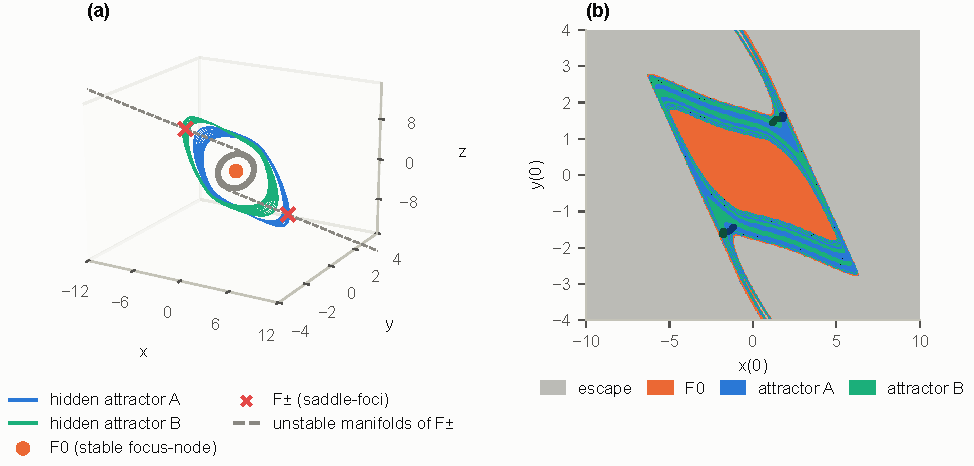
\includegraphics[width=\textwidth]{figures/fig30_chua_I_hidden.pdf}
\caption{Chua circuit, parameter set I. (a) Two symmetric hidden chaotic attractors A and B, the stable focus-node F$_0$ (dot), the saddle-foci F$_\pm$ (crosses), and their unstable manifolds. One branch of each manifold escapes to infinity and the other winds onto F$_0$, so the standard procedure does not find attractors A and B. (b) Basins in the plane $z(0)=0$ (window $|y|\le4$). Gray: escape to infinity; orange: F$_0$; blue and green: attractors A and B.}
\label{fig:chuaI}
\end{figure*}

\begin{figure}
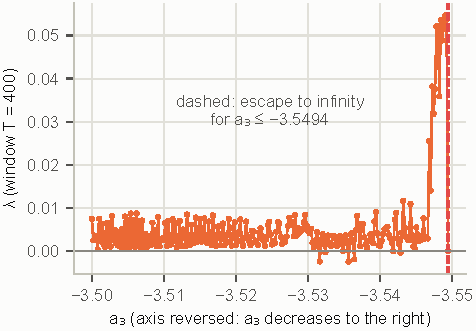
\includegraphics[width=\columnwidth]{figures/fig35_jafari2026.pdf}
\caption{System of Jafari \textit{et al.}\cite{Jafari2026NoPP} without fixed and perpetual points: the Lyapunov exponent over windows $T=400$ in the narrow chaos window near the boundedness limit ($a_3$ decreases to the right); for $a_3\le-3.5494$, trajectories escape to infinity. The cycle at $a_3=-1$ and the chaotic attractor at $a_3=-3.548$ are shown in Fig.~\ref{fig:gallery3d}.}
\label{fig:jafari}
\end{figure}

\begin{figure*}
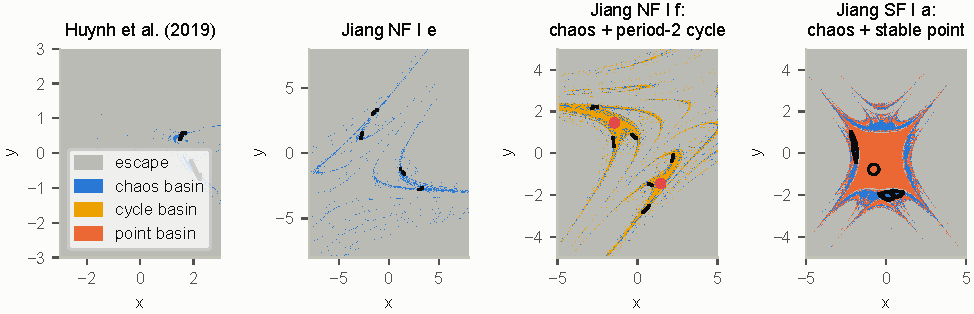
\includegraphics[width=\textwidth]{figures/fig34_maps_phase_basin.pdf}
\caption{Two-dimensional maps of level B: phase--basin portraits. (a) The map of Huynh \textit{et al.}\cite{Huynh2019} without fixed points ($p=0.0091$ in $[-3,3]^2$). (b), (c) Cases NF~I~e and NF~I~f of the family of Jiang \textit{et al.}\cite{Jiang2016Maps} without fixed points; in NF~I~f, a chaotic attractor coexists with a period-2 cycle (markers). (d) Case SF~I~a with a single stable fixed point (circle). Light gray: escape; dark blue: basin of the chaotic attractor; white: basin of the cycle; orange: basin of the fixed point; black: the attractor.}
\label{fig:maps}
\end{figure*}

\begin{figure*}
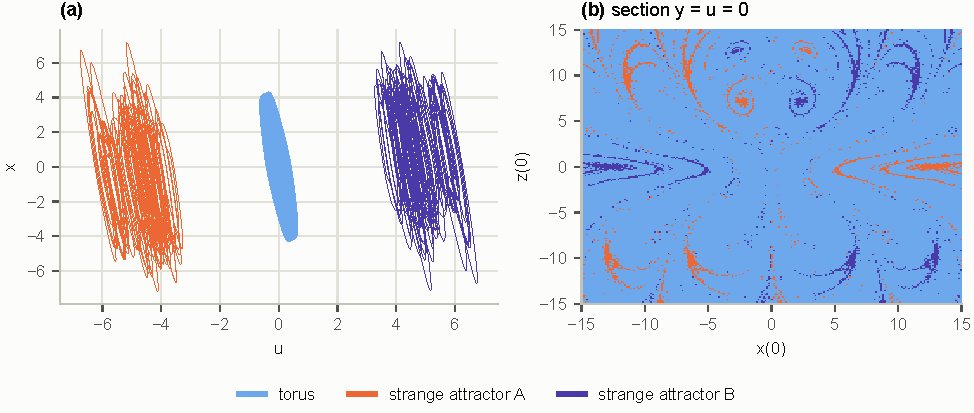
\includegraphics[width=\textwidth]{figures/fig33_li_sprott_4d.pdf}
\caption{Four-dimensional simplified Lorenz system\cite{LiSprott2014} at $a=6$, $b=0.1$; there are no equilibria. (a) The torus (basin fraction 0.090) and a pair of symmetric strange attractors ($\lambda\approx0.25$; 0.446 and 0.464) in the projection $(u,x)$. (b) Basins in the section $y=u=0$ of the box $[-15,15]^4$; the torus occupies the ``background,'' and the strange attractors form spiral tongues. Here the rare target is the torus, not the chaos.}
\label{fig:levelA}
\end{figure*}

\section{Verification episodes}\label{app:verification}

This appendix documents the three cases mentioned in Sec.~\ref{sec:protocol} and the measured hiddenness.

\textbf{Numerical ``transient chaos'' in the Chua circuit.} With RK4 at $\Delta t=0.01$, all 256 copies of a state on the hidden chaotic set of Chua~I converge within $t\le2\times10^4$ to a spurious periodic orbit of the same size (median time about 1500; Fig.~\ref{fig:chuatrans}a). At $\Delta t=0.0025$, none of 96 copies leaves before $t=10^4$, and DOP853 preserves the chaos up to $t=4000$. At $\Delta t=0.01$, the fractions of the hidden attractors are underestimated almost twofold (Fig.~\ref{fig:chuatrans}b). For a piecewise-linear system, this is an integrator artifact and the mirror image of the spurious ``hidden Lorenz attractor'':\cite{Munmuangsaen2018,SprottMunmuangsaen2018Comment} there, transient chaos was mistaken for an attractor; here, an attractor is mistaken for transient chaos. The step-convergence check is therefore mandatory.

\textbf{Basin fractions of the Chua circuit.} Two independent implementations, Python (RK4, $\Delta t=0.0025$) and Attractors.jl (Vern9), give identical fractions in the balls $r=3$ and $r=5$ and in Zelinka's box. Neither of them reproduces Table~1 of the review in Ref.~\onlinecite{GuanXie2025} (Table~\ref{tab:chuafrac}). In the ball $r=3$, the escape fraction is 0.19 in our computations versus 0.06 in the review, the fraction of F$_0$ is 0.44 versus 0.75, and that of each hidden attractor is 0.18 versus 0.095. The last pair is suggestive: our fractions of the hidden attractors at the coarse step $\Delta t=0.01$ are also about 0.09 (Fig.~\ref{fig:chuatrans}b), so the review's values are consistent with the artifact above, whereas its escape and F$_0$ fractions remain unexplained. The basin structure in the plane $z=0$ coincides with the review and with the catalog of Ref.~\onlinecite{Wagemakers2025Zoo} (Fig.~\ref{fig:chuaI}).

\textbf{Intermittency and transient sets.} In NE4, the ``second attractor'' of a preliminary version of the protocol turned out to be intermittency of the single chaotic attractor; this was fixed by the window $T_{\rm obs}=500\gg1/\lambda$. The transient chaos of the Lorenz system $(4,29,2)$ lives about $10^4$ time units: all eight copies decay by $t\le7\times10^4$. A protocol with an observation window shorter than the lifetime would accept this set as an attractor (Fig.~\ref{fig:verif}). The Rabinovich set at $r=6.8$ lives longer than $10^5$ for six of eight copies, consistent with the estimate $\tau\sim5\times10^7$ of Ref.~\onlinecite{SprottMunmuangsaen2018Comment}; in the benchmark, it is used only as a control.

\textbf{Hiddenness measure.} Table~\ref{tab:hidden} lists $h_\varepsilon$ for the systems with equilibria. For SE3 and SE11, $h_\varepsilon=0$ at all three scales. For Chua~I, $h_\varepsilon$ grows from 0 at $\varepsilon=10^{-3}L$ through 0.003 ($10^{-2}L$) to 0.19 ($10^{-1}L$). For the Rabinovich system at $r=100$, the values are 0, 0.03, and 0.65: the attractor is hidden only in the strict limit $\varepsilon\to0$, and already at $\varepsilon=10^{-2}L$, trajectories from the neighborhood of an equilibrium enter its basin. The binary definition thus does not distinguish ``deeply'' and ``shallowly'' hidden attractors, whereas $h_\varepsilon$ does. For the Jafari chaos, whose copies with a perturbation of $10^{-3}$ escape (Fig.~\ref{fig:verif}), all 32 copies with a perturbation of $10^{-6}$ stay on the attractor for $10^4$ time units with RK4, and so do eight copies with DOP853, with finite-time exponents of $0.056\pm0.011$ and none below 0.01: it is an attractor with a basin thinner than a relative distance of $10^{-3}$ near the attractor, not a long transient.

A measured zero of $h_\varepsilon$ is informative only relative to the number of starts $n$: with no hits, $h_\varepsilon<3/n$ at the 95\% level, so the zeros of Table~\ref{tab:hidden} bound $h_\varepsilon$ by the values given there, and for the rare targets with $p$ comparable to $3/n$ the zero does not by itself separate ``hidden'' from ``rare.'' For SE11, Chua~II, and the rare family of the coupled Chua circuits, the measure was therefore remeasured with $2\times10^5$ starts per radius: no start reaches a hidden target at $10^{-3}L$ or $10^{-2}L$, so $h_\varepsilon<1.5\times10^{-5}$ at the 95\% level, below the basin measures of all three targets (Sec.~\ref{sec:coupled}).

% Proposed caption (replaces the bar chart fig04_table1_comparison / \ref{fig:table1}):
% Basin fractions of Chua~I under uniform sampling in balls of radius $r=3$ and $r=5$ about the origin: escape to infinity ($\infty$), the stable equilibrium F$_0$, and the two symmetric hidden attractors A and B. Sources: Table~1 of the review in Ref.~\onlinecite{GuanXie2025} and two independent implementations, Python (RK4, $dt=0.0025$, $10^5$ points per ball) and Attractors.jl (Vern9, $10^4$ points per ball). The two implementations agree with each other but not with the review. In the implementations, A and B are matched by the sign of the mean of $x$ on the attractor; for the review, they are listed in the order of its Table~1. The fraction of unmatched trajectories in the Python run (0.06\%) is omitted.

\begin{table}
\caption{Basin fractions of Chua~I under uniform sampling in balls of radius $r=3$ and $r=5$ about the origin: escape to infinity ($\infty$), the stable equilibrium F$_0$, and the two symmetric hidden attractors A and B. Sources: Table~1 of the review in Ref.~\onlinecite{GuanXie2025} and two independent implementations, Python (RK4, $dt=0.0025$, $10^5$ points per ball) and Attractors.jl (Vern9, $10^4$ points per ball). The two implementations agree with each other but not with the review. In the implementations, A and B are matched by the sign of the mean of $x$ on the attractor; for the review, they are listed in the order of its Table~1. The fraction of unmatched trajectories in the Python run (0.06\%) is omitted.}
\label{tab:chuafrac}
\footnotesize
\setlength{\tabcolsep}{3pt}
\begin{ruledtabular}
\begin{tabular}{lrrrrrrrr}
 & \multicolumn{4}{c}{$r=3$} & \multicolumn{4}{c}{$r=5$} \\
Source & $\infty$ & F$_0$ & A & B & $\infty$ & F$_0$ & A & B \\
\hline
Ref.~\onlinecite{GuanXie2025}, Table~1 & 0.06 & 0.75 & 0.09 & 0.10 & 0.23 & 0.50 & 0.14 & 0.13 \\
Python, RK4 & 0.19 & 0.44 & 0.18 & 0.18 & 0.55 & 0.18 & 0.14 & 0.14 \\
Attractors.jl & 0.19 & 0.44 & 0.18 & 0.19 & 0.55 & 0.18 & 0.13 & 0.14 \\
\end{tabular}
\end{ruledtabular}
\end{table}


% Proposed caption (replaces the plot fig40_hiddenness / \ref{fig:hidden}):
% Hiddenness measure $h_\varepsilon$: the fraction of trajectories started in the $\varepsilon$-neighborhoods of the equilibria (uniformly in the ball of radius $\varepsilon$ about each equilibrium, plus the two points $e\pm\varepsilon u$ along every unstable eigendirection $u$) that enter the basin of the attractor, for $\varepsilon=10^{-3}L$, $10^{-2}L$, and $10^{-1}L$, where $L$ is the half-width of the region $B$; $n$ is the number of starts per radius. An entry 0 means no hit among the $n$ starts (95\% upper bound $3/n$). For Chua~I and Chua~II, the two hidden attractors are listed separately; the values quoted in the text for Chua~I are the sums over A and B. The Lorenz transient set is shown for comparison.
% Data caveat (results/e11_hiddenness.json): the reference set of this experiment contains one chaotic attractor of Chua II
% (new1) and the cycle LC (new0); at eps = 1e-1 L, 103 of 1202 starts (8.6%) reach an unmatched regime, presumably the
% symmetric second chaotic attractor, so h for "chaos, both" would be about 0.18. Wang--Chen #2 at 1e-1 L: 2 unmatched, 1% escape.
% Hits behind the nonzero entries: Chua I A 3/101, B 1/122 (1e-2 L / 1e-1 L); Chua II LC 484, chaos 115; Rabinovich 39/781;
% Lorenz 49.

\begin{table}
\caption{Hiddenness measure $h_\varepsilon$: the fraction of trajectories started in the $\varepsilon$-neighborhoods of the equilibria (uniformly in the ball of radius $\varepsilon$ about each equilibrium, plus the two points $e\pm\varepsilon u$ along every unstable eigendirection $u$) that enter the basin of the attractor, for $\varepsilon=10^{-3}L$, $10^{-2}L$, and $10^{-1}L$, where $L$ is the half-width of the region $B$; $n$ is the number of starts per radius. An entry 0 means no hit among the $n$ starts (95\% upper bound $3/n$). For Chua~I and Chua~II, the two hidden attractors are listed separately; the values quoted in the text for Chua~I are the sums over A and B. The Lorenz transient set is shown for comparison.}
\label{tab:hidden}
\footnotesize
\begin{ruledtabular}
\begin{tabular}{lrrrr}
System, attractor & $n$ & $\varepsilon=10^{-3}L$ & $10^{-2}L$ & $10^{-1}L$ \\
\hline
Chua I, A & 1204 & 0 & 0.00249 & 0.0839 \\
Chua I, B & 1204 & 0 & 0.000831 & 0.101 \\
Chua II, cycle LC & 1202 & 0 & 0 & 0.403 \\
Chua II, chaos & 1202 & 0 & 0 & 0.0957 \\
Wang--Chen \#2 & 400 & 0 & 0 & 0.838 \\
SE3 & 400 & 0 & 0 & 0 \\
SE11 & 400 & 0 & 0 & 0 \\
Rabinovich, $r=100$ & 1202 & 0 & 0.0324 & 0.650 \\
Lorenz $(4,29,2)$, transient set & 1202 & 0 & 0 & 0.0408 \\
\end{tabular}
\end{ruledtabular}
\end{table}


\begin{figure}
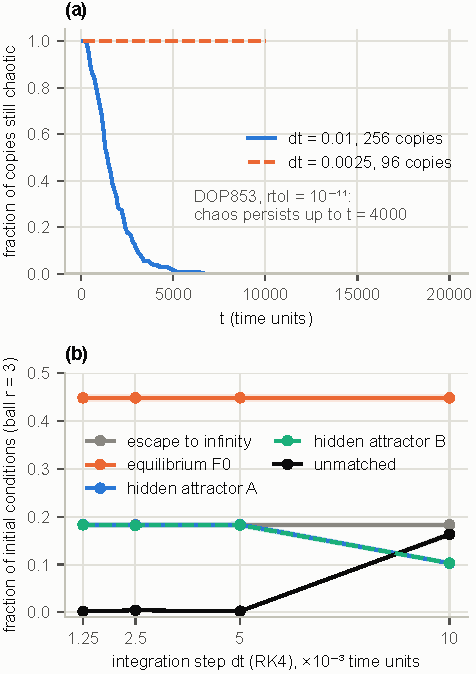
\includegraphics[width=\columnwidth]{figures/fig02_chua_transient.pdf}
\caption{Numerical ``transient chaos'' in Chua~I. (a) The fraction of copies (initial perturbation $10^{-3}$) remaining on the hidden chaotic set. With RK4 at $\Delta t=0.01$, the chaos decays onto a spurious periodic orbit; at $\Delta t=0.0025$, it persists to the end of the window. (b) Basin fractions versus the RK4 step (ball $r=3$, $2\times10^4$ points, $T_{\rm tr}=1000$). At $\Delta t=0.01$, about 16\% of trajectories land on the spurious orbit (``unmatched''), and the fractions of the hidden attractors are underestimated. For $\Delta t\le0.005$, the fractions stabilize.}
\label{fig:chuatrans}
\end{figure}

\begin{figure*}
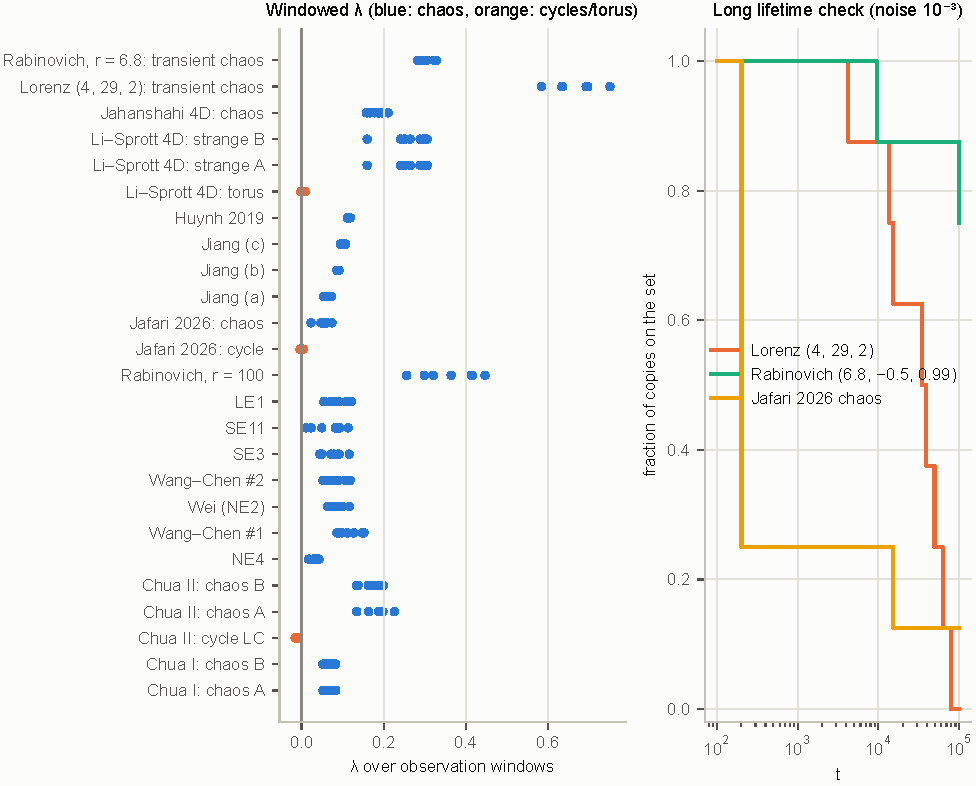
\includegraphics[width=\textwidth]{figures/fig41_verification.pdf}
\caption{Verification of the targets. (a) The largest Lyapunov exponent over consecutive observation windows for all targets of the benchmark; blue: chaotic regimes; orange: regular ones (cycle LC of Chua~II, the Jafari cycle, the Li--Sprott torus). (b) Long lifetime check (eight copies with initial perturbation $10^{-3}$). The Lorenz transient chaos decays completely. For the Rabinovich set at $r=6.8$, six of eight copies survive to $10^5$. For the fragile Jafari chaos, six of eight copies escape to infinity already by $t=200$: with a relative perturbation of $10^{-3}$, the copies leave its thin basin; with $10^{-6}$, all of them stay on the attractor (Appendix~\ref{app:verification}).}
\label{fig:verif}
\end{figure*}

\section{Classical heuristics}\label{app:classic}

The classical heuristics behave on the benchmark in agreement with the review in Ref.~\onlinecite{GuanXie2025} (Table~\ref{tab:classic}). Perpetual points lead to the target in Wang--Chen \#1, Wei, and Rabinovich. The Chua circuit has none: in the linear zones, the acceleration vanishes only at equilibria. They are also absent in SE3, SE11, and Wang--Chen \#2, while in NE4 and LE1 they exist but do not lead to the target. Sampling on nullclines (coordinate-wise zero-velocity sets\cite{Godara2018CVS}) gives gains in hit frequency from 1.1 (SE11) and 2.6 (LE1) to 4.5 (Chua~I). Connecting curves\cite{GuanXie2021CC} gain a factor of 2 in Wang--Chen \#1 and give no hits in SE3 and SE11. Continuation from the describing function finds the target in Chua~I within 10 integrations but applies only to Lur'e-type systems.

% Proposed caption (replaces the bar chart fig07_classic_vs_uniform / \ref{fig:classic}):
% Classical heuristics versus uniform sampling on the level-A targets: the number of integrations to detection with probability 0.9, $N_{0.9}=\lceil\ln0.1/\ln(1-p)\rceil$, where $p$ is the hit frequency of the sampling scheme. Uniform: sampling in $B$ ($p$ from $2\times10^4$ points; the geometric value, which differs slightly from the measured $N^0_{0.9}$ of Table~\ref{tab:gains}). CVS: sampling on the coordinate-wise zero-velocity sets (nullclines) $\dot x_i=0$, up to $10^3$ points on each, best coordinate. CC: sampling on connecting curves, 400 points. ``Not found'': no hit among the sampled points. PP: the number of perpetual points that lead to the target over the number of perpetual points found (``none'': the system has no perpetual points).

\begin{table}
\caption{Classical heuristics versus uniform sampling on the level-A targets: the number of integrations to detection with probability 0.9, $N_{0.9}=\lceil\ln0.1/\ln(1-p)\rceil$, where $p$ is the hit frequency of the sampling scheme. Uniform: sampling in $B$ ($p$ from $2\times10^4$ points; the geometric value, which differs slightly from the measured $N^0_{0.9}$ of Table~\ref{tab:gains}). CVS: sampling on the coordinate-wise zero-velocity sets (nullclines) $\dot x_i=0$, up to $10^3$ points on each, best coordinate. CC: sampling on connecting curves, 400 points. ``Not found'': no hit among the sampled points. PP: the number of perpetual points that lead to the target over the number of perpetual points found (``none'': the system has no perpetual points).}
\label{tab:classic}
\footnotesize
\setlength{\tabcolsep}{3pt}
\begin{ruledtabular}
\begin{tabular}{lrrrr}
Target & Uniform & CVS & CC & PP \\
 & $N^0_{0.9}$ & $N_{0.9}$ & $N_{0.9}$ & hits/total \\
\hline
Rabinovich, $r=100$ & 2 & 2 & 2 & 2/2 \\
Wang--Chen \#2 & 3 & 1 & 2 & none \\
NE4 & 6 & 7 & 29 & 0/1 \\
SE3 & 14 & 11 & not found & none \\
Wang--Chen \#1 & 22 & 19 & 11 & 1/2 \\
Wei (NE2) & 23 & 17 & 22 & 1/2 \\
Chua I, chaos A\footnotemark[1] & 136 & 14 & 172 & none \\
Chua I, chaos B\footnotemark[1] & 124 & 14 & 172 & none \\
SE11 & 291 & 255 & not found & none \\
LE1 & 1475 & 575 & 920 & 0/1 \\
\end{tabular}
\end{ruledtabular}
\footnotetext[1]{The heuristics count hits on either of the two hidden attractors; the uniform cost for either attractor is 65.}
\end{table}


\section{Ablation, baselines, and robustness}\label{app:ablation}

\textbf{Ablation.} The contributions of the components are shown in Fig.~\ref{fig:ablation}. On Chua~II, the arms add up: the portfolio gives 7.4 times, versus 5.1 for splitting and 3.2 for active learning. On LE1, the active-learning arm hurts, and the gain of the portfolio is provided by the splitting arm. Without the uniform share, the portfolio is not faster (Chua~II: 7.0; SE11: 3.1; LE1: 5.1) and loses where there is no signal (Jafari cycle: 0.27 against 0.43). On LE1, the lower interval bound for $G$ without the uniform share is 1.59, whereas for the portfolio with $\theta=0.2$, it is 3.76. Multidimensional ``rarity'' as a reaction coordinate produces heavy tails: the chains get stuck in atypical but nontarget regions, for example, in the basin of an equilibrium inside the D2 ball. The escape step as a coordinate is equivalent to $\xi$ everywhere except Chua~II, where all trajectories are bounded and it gives 1.04 against 5.05. Two earlier strategies were also tested ($R=20$): adaptive multilevel splitting driven by the novelty of the asymptotic fingerprint finds the target on Chua~II in only 55\% of runs, and MAP-Elites with the fingerprint as behavior descriptor has a median 5.6 times better than uniform sampling but a heavy tail, $G=0.36$. Such tails are what the uniform share of the portfolio removes.

\begin{figure*}
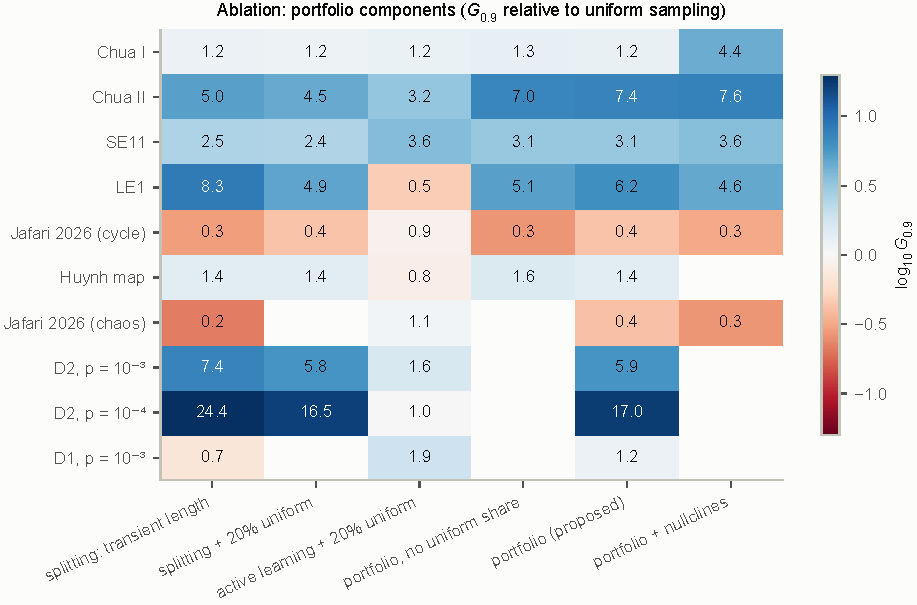
\includegraphics[width=\textwidth]{figures/fig25_ablation.pdf}
\caption{Ablation: $G_{0.9}$ of the variants of the method relative to uniform sampling ($R=100$; color: $\log_{10}G$; empty cells: the variant was not run). Rows: systems of levels A and B and synthetic families; columns: splitting alone and with a uniform share, active learning with a uniform share, the portfolio without a uniform share, the portfolio, and the portfolio with nullclines. Columns 1, 3, 5, and 6 repeat Table~\ref{tab:gains}; the new information is in columns 2 and 4 and in the D1 and D2 rows.}
\label{fig:ablation}
\end{figure*}

% Differential-evolution baseline: exact description of the implementation
% (src/hsearch/search/strategies.py, class DEZelinka; harness in src/hsearch/search/harness.py;
% configuration in experiments/e50_batch_runner.py and e20_search_benchmark.py).
% One paragraph, no table; intended for the appendix.

\textbf{Differential-evolution baseline.} The baseline is differential evolution over initial conditions with the cost function of Ref.~\onlinecite{Zelinka2016}, in the variant DE/rand/1/bin used there. The population has $N_P=25$ members (half of the initial sample $n_0=50$ of the other strategies, but not fewer than 10), the differential weight is $F=0.9$, and the crossover probability is $C_R=0.3$, the values of Ref.~\onlinecite{Zelinka2016}. The initial population is drawn uniformly from the region $B$ and consists of the first 25 points of the uniform stream of the run, so that it coincides with the first 25 points of uniform sampling (common random numbers). In every generation, for each member $x_i$, three other members $x_{r_1}$, $x_{r_2}$, $x_{r_3}$, distinct from one another and from $x_i$, are drawn without replacement; the mutant is $v=x_{r_3}+F\,(x_{r_1}-x_{r_2})$; the trial $u_i$ takes each coordinate from $v$ with probability $C_R$ and from $x_i$ otherwise, with one randomly chosen coordinate always taken from $v$; and $u_i$ is clipped to $B$ coordinate by coordinate. The 25 trials of a generation form one batch and are integrated with the full protocol ($T_{\rm tr}+T_{\rm obs}$ of Table~\ref{tab:integration}); $u_i$ replaces $x_i$ if its cost is not larger than that of $x_i$. The cost is computed from the trajectory fingerprint alone: with $r_{\max}$ the maximum of the Euclidean norm of the state over the observation window $T_{\rm obs}$ (after the transient $T_{\rm tr}$), the cost is 0 if $d_{\rm lo}\le r_{\max}\le d_{\rm hi}$ and $r_{\max}$ otherwise, and it is $10^6$ for a trajectory that escapes beyond $R_{\rm esc}$ or produces a non-finite state at any time. This is the function of Ref.~\onlinecite{Zelinka2016}, where the maximum is taken over the last 50 time units of a run of length 200 and the interval $[d_{\rm lo},d_{\rm hi}]=[3,11]$ was chosen empirically for the hidden attractor of the Chua circuit; the pair $(3,11)$ remains the default of the implementation but is not used in the benchmark. Instead, the interval is set from the size of the target, which is the sense in which the baseline is ``told the size'': if $r^\ast$ denotes the value of $r_{\max}$ in the fingerprint of the target reference (the mean over its 64 calibration copies; for a problem with several target regimes, the largest of their values), then $[d_{\rm lo},d_{\rm hi}]=[0.5\,r^\ast,\,1.5\,r^\ast]$. For Chua~I, $r^\ast=10.9$ and the interval is $[5.5,16.4]$. The cost does not use the labels of the identification protocol, so the search does not distinguish the target from any other bounded regime whose size falls into the interval. Budget and detection are the same as for every other strategy: each integrated trial counts as one evaluation, the initial population included; a run has the per-problem budget of Sec.~\ref{sec:measure} (5--15 times $N^0_{0.9}$ on levels A and B, from $10^3$ integrations on Chua~I to $4\times10^4$ on the Jafari chaos); and the first hit is the ordinal number, in the order of evaluation, of the first integrated point whose fingerprint the identification protocol matches to the target reference, whether or not that point is accepted into the population. The run stops at the end of the generation in which the hit occurs, and $N_{0.9}$ is the 0.9 quantile of the first-hit number over the $R$ runs.


\textbf{Bisection toward basin boundaries.} A natural alternative that uses basin boundaries directly is bisection toward them, in the spirit of edge tracking\cite{Skufca2006Edge,Schneider2007Edge} and of the straddle method.\cite{NusseYorke1989} A chain starts from a point with a long transient and the nearest point of another class and halves the segment between them 12 times; new chains start as old ones end. Bisection is a strong baseline on systems with smooth boundaries (Table~\ref{tab:bisection}): it gives 4.2 on SE11 (portfolio: 3.1), 6.0 on LE1 (6.2), 1.3 on Chua~I (1.2), and 3.6 on D1 at $p=10^{-3}$ (1.2). It loses where the signal is graded over many scales: 3.1 on Chua~II (7.4) and 1.6 and 1.3 on D2 at $p=10^{-3}$ and $10^{-4}$ (5.9 and 17). On the problems without a signal, bisection stays near 1 (0.96--1.18), whereas the portfolio pays for its arms (0.42--0.43). On the coupled copies of SE11, it does not scale (Sec.~\ref{sec:coupled}). Bisection as a fourth arm of the portfolio, with fixed or adaptive shares, helps only where bisection alone is strong (in $R=50$ runs: D1 at $p=10^{-3}$, 1.7 against 1.2; LE1, 8.6 against 6.2) and takes budget from splitting on the problems with the largest gains (three coupled copies of SE11 at $R=20$: 1360 against 1570). We therefore retain the three-arm portfolio.

\begin{table}
\caption{Bisection toward basin boundaries ($R=50$) and the portfolio ($R=100$, from Tables~\ref{tab:gains} and \ref{tab:scaling}): gains $G_{0.9}$ with 95\% bootstrap intervals. Bold: values whose lower interval bound exceeds 1. A lower bound of 0 means that some bootstrap resamples did not reach 90\% success.}
\label{tab:bisection}
\footnotesize
\begin{ruledtabular}
\begin{tabular}{lrr}
Problem & Bisection & Portfolio \\
\hline
Chua I & \textbf{1.30} \ci{1.06}{1.95} & 1.24 \ci{0.94}{1.77} \\
Chua II & \textbf{3.14} \ci{1.69}{5.12} & \textbf{7.36} \ci{6.09}{10.2} \\
SE11 & 4.17 \ci{0}{4.64} & \textbf{3.10} \ci{2.46}{3.70} \\
LE1 & \textbf{6.02} \ci{4.47}{9.57} & \textbf{6.24} \ci{3.76}{10.0} \\
Jafari 2026, cycle & 0.96 \ci{0.53}{1.61} & 0.43 \ci{0.29}{0.78} \\
Huynh 2019 & 1.05 \ci{0.37}{2.21} & \textbf{1.40} \ci{1.16}{2.54} \\
Jafari 2026, chaos & 1.18 \ci{0.77}{2.06} & 0.42 \ci{0.29}{0.58} \\
D2, $p=10^{-3}$ & 1.64 \ci{1.00}{2.52} & \textbf{5.88} \ci{5.02}{8.10} \\
D2, $p=10^{-4}$ & 1.29 \ci{0}{1.82} & \textbf{17.0} \ci{13.6}{22.2} \\
D1, $p=10^{-3}$ & \textbf{3.62} \ci{2.84}{4.89} & 1.19 \ci{0.86}{1.58} \\
\end{tabular}
\end{ruledtabular}
\end{table}

\textbf{Stagger-and-step.} The splitting arm is a multichain relative of the stagger-and-step method,\cite{SweetNusseYorke2001} which locates chaotic saddles by climbing the escape time of a single trajectory with random perturbations of log-uniformly distributed size. We ran a stagger-and-step search with the same reaction coordinate: a single chain keeps the point with the largest $\xi$, proposes a perturbation in a random direction with a size log-uniform between $10^{-3}$ and 1 of the region width, accepts it when $\xi$ increases, and restarts from a uniform point after 30 consecutive rejections; full integration and the budgets of Table~\ref{tab:gains} were used ($R=50$; three coupled copies of SE11: $R=20$). The results are in Table~\ref{tab:stagger}. Where the coordinate carries a signal, stagger-and-step is the strongest strategy of the paper: 1.7 on Chua~I, 10 on Chua~II, and from 2.1 to 155 on D2 at $p=10^{-2}$--$10^{-5}$, with a scaling exponent $s=0.32$ [0.28, 0.37] against 0.45 for the portfolio and 0.41 for splitting; on SE11, LE1, and three coupled copies of SE11, it is comparable with the portfolio (2.9, 5.9, and 735 against 3.1, 6.2, and 1435). Where the coordinate is deceptive or uninformative, it fails, and without a uniform share it falls below the bound of the portfolio: 0.16 on the Jafari cycle, 0.26 on the Jafari chaos, and 0.93 on the Huynh map, and on D1 it finds the target within six times the uniform cost in only 60\% of the runs. The gain thus comes from the reaction coordinate rather than from the way of climbing it, and the contribution of the portfolio is the bound. A stagger-and-step chain is a natural arm of the portfolio that would combine its efficiency with the guarantee; we leave this combination to future work.

\begin{table}
\caption{Stagger-and-step\cite{SweetNusseYorke2001} on the reaction coordinate $\xi$ against splitting and the portfolio: gains $G_{0.9}$ relative to the uniform reference of Tables~\ref{tab:gains}--\ref{tab:coupled}, with 95\% bootstrap intervals over the stagger runs. Bold: lower interval bound above 1; ``---'' with a percentage: fewer than 90\% of the runs found the target within the budget.}
\label{tab:stagger}
\footnotesize
\setlength{\tabcolsep}{3pt}
\begin{ruledtabular}
\begin{tabular}{lrrrr}
Problem & $R$ & Stagger-and-step & Splitting & Portfolio \\
\hline
%TABSTAGGER-BEGIN
Chua I & 50 & \textbf{1.67} \ci{1.02}{2.20} & 1.20 & 1.24 \\
Chua II & 50 & \textbf{10.1} \ci{8.80}{13.1} & 5.05 & 7.36 \\
SE11 & 50 & \textbf{2.90} \ci{1.71}{3.69} & 2.53 & 3.10 \\
LE1 & 50 & \textbf{5.85} \ci{3.77}{8.86} & 8.29 & 6.24 \\
Jafari 2026, cycle & 50 & 0.16 \ci{0.14}{0.26} & 0.29 & 0.43 \\
Huynh 2019 & 50 & 0.93 \ci{0.63}{1.45} & 1.36 & 1.40 \\
Jafari 2026, chaos & 50 & 0.26 \ci{0.23}{0.36} & 0.22 & 0.42 \\
D1, $p=10^{-3}$ & 20 & --- (60\%) & 0.69 & 1.19 \\
D2, $p=10^{-2}$ & 50 & \textbf{2.14} \ci{1.93}{2.90} & 2.29 & 2.27 \\
D2, $p=10^{-3}$ & 50 & \textbf{6.99} \ci{5.32}{9.07} & 7.37 & 5.87 \\
D2, $p=10^{-4}$ & 50 & \textbf{34.5} \ci{31.3}{50.9} & 24.4 & 17.0 \\
D2, $p=10^{-5}$ & 50 & \textbf{155} \ci{120}{187} & 93.1 & 72.0 \\
3 coupled SE11 & 20 & \textbf{735} \ci{237}{1357} & 682 & 1435 \\
%TABSTAGGER-END
\end{tabular}
\end{ruledtabular}
\end{table}

\textbf{Robustness.} The hyperparameters of the portfolio were not tuned to the problems: everywhere $\theta=0.2$, $p_0=0.2$, $\sigma_0=0.1$, and $n_0=50$. Each of them was varied separately on three problems with a gain ($R=50$; Table~\ref{tab:robust}). No variant brings the gain below 1: on Chua~II, it lies in the range 5.2--7.5; on D2, 14.7--21.8; and on LE1, 3.1--9.2. A larger initial sample ($n_0=100$) worsens the gain on targets with $p\sim10^{-3}$, where the initial sample is a noticeable part of the cost, and improves it on D2 ($p=10^{-4}$). Scaling both integration windows by 0.5 and 2 on Chua~II, SE11, LE1, and D2 ($p=10^{-4}$) changed the cost of uniform sampling by at most 12\% and kept the gains within a factor of 1.7 of the base values: 7.0 and 6.3 on Chua~II (base 7.4), 3.8 and 3.6 on SE11 (3.1), 3.6 and 6.7 on LE1 (6.2), and 18 and 18 on D2 (17).

\begin{table*}
\caption{Robustness of the portfolio to hyperparameters: $G_{0.9}$ with 95\% bootstrap intervals (variants: $R=50$; base: $R=100$). In each column, one parameter is changed relative to the base set $\theta=0.2$, $p_0=0.2$, $\sigma_0=0.1$, $n_0=50$.}
\label{tab:robust}
\footnotesize
\begin{ruledtabular}
\begin{tabular}{lrrrrrrr}
Problem & Base & $\theta=0.1$ & $\theta=0.3$ & $p_0=0.1$ & $p_0=0.3$ & $\sigma_0=0.3$ & $n_0=100$ \\
\hline
Chua II & 7.36 \ci{6.09}{10.2} & 6.90 \ci{5.27}{10.4} & 5.70 \ci{4.58}{8.24} & 7.53 \ci{6.31}{11.7} & 6.32 \ci{5.23}{8.87} & 5.23 \ci{4.23}{8.29} & 5.23 \ci{4.27}{7.79} \\
LE1 & 6.24 \ci{3.76}{10.0} & 6.86 \ci{4.07}{13.3} & 6.48 \ci{3.34}{10.9} & 9.16 \ci{1.96}{14.7} & 6.85 \ci{4.96}{10.8} & 3.15 \ci{2.39}{6.85} & 3.12 \ci{2.11}{5.45} \\
D2, $n=6$, $p=10^{-4}$ & 17.0 \ci{13.6}{22.2} & 14.7 \ci{10.6}{24.1} & 18.5 \ci{13.2}{24.7} & 21.8 \ci{14.4}{36.2} & 18.8 \ci{13.9}{27.8} & 18.2 \ci{13.7}{26.5} & 20.7 \ci{11.1}{28.2} \\
\end{tabular}
\end{ruledtabular}
\end{table*}

\section{Real systems in enlarged regions}\label{app:enlarged}

To test whether the gain grows on real systems as $p$ decreases, we enlarged the region of initial conditions $k$ times about its center, $B_k=kB$ with $k=2$--16, keeping the escape radius at least twice the distance to the farthest corner. If the basin lay inside $B$, its measure in $B_k$ would be $p_{k=1}/k^3$. It is not (Table~\ref{tab:enlarged}, Fig.~\ref{fig:enlarged}a): for SE11, $p$ falls from $7.7\times10^{-3}$ only to $2.4\times10^{-4}$ at $k=16$, against $1.9\times10^{-6}$ expected, and the other systems behave similarly. The basins of these hidden attractors extend far beyond $B$, so their rarity is a property of the chosen region rather than of the attractor. Continuation of the hidden attractors in a parameter gives the same conclusion: in Chua~II, the Wang--Chen and Wei systems, the basin fraction stays at $10^{-3}$--$0.7$ up to the crisis at which the attractor disappears, and in LE1 it falls to $2.4\times10^{-4}$ at most. Over the enlarged regions, the gain grows as $p$ decreases on three of the five systems (Fig.~\ref{fig:enlarged}b): on SE11, from 3.1 to 24; on LE1, from 6.2 to 16; and on Chua~I, from 1.2 to 6.3. The effective exponents of these growths, $\ln G/\ln(p_{k=1}/p)$, are 0.4--0.7, with the caveat that the enlargement changes the geometry of the basin as well as its measure. On Chua~II, the gain falls from 7.4 to 0.71 at $k=4$, and splitting alone falls to 0.14, because the longest transients belong to trajectories that return slowly from far away rather than to the neighborhood of the target. On the Jafari cycle, where there is no signal, the portfolio stays at 0.24--0.43, within the guarantee.

\begin{table*}
\caption{Real systems in the enlarged regions $kB$ ($R=50$; $k=1$: $R=100$): basin measure, cost of uniform sampling, and gains $G_{0.9}$ with 95\% bootstrap intervals. Bold: values whose lower interval bound exceeds 1; a lower bound of 0 means that some bootstrap resamples did not reach 90\% success; ``---'' with a percentage: fewer than 90\% of the runs found the target.}
\label{tab:enlarged}
\footnotesize
\setlength{\tabcolsep}{3pt}
\begin{ruledtabular}
\begin{tabular}{lrrrrr}
System & $k$ & $p$ & $N^0_{0.9}$ & Splitting & Portfolio \\
\hline
SE11 & 1 & 0.0077 & 317 & \textbf{2.53} \ci{1.95}{2.86} & \textbf{3.10} \ci{2.46}{3.70} \\
SE11 & 2 & 0.0023 & 811 & \textbf{3.91} \ci{3.03}{4.66} & \textbf{4.93} \ci{3.96}{6.01} \\
SE11 & 4 & $6.1\times10^{-4}$ & 3858 & \textbf{11.8} \ci{6.38}{19.4} & \textbf{17.5} \ci{8.95}{26.8} \\
SE11 & 8 & $4.5\times10^{-4}$ & 5191 & \textbf{9.92} \ci{5.54}{14.5} & \textbf{9.19} \ci{5.87}{17.0} \\
SE11 & 16 & $2.4\times10^{-4}$ & 9351 & \textbf{15.8} \ci{9.96}{21.8} & \textbf{24.2} \ci{13.8}{34.5} \\
LE1 & 1 & 0.0013 & 1617 & \textbf{8.29} \ci{6.35}{12.3} & \textbf{6.24} \ci{3.76}{10.0} \\
LE1 & 2 & $5.3\times10^{-4}$ & 4540 & \textbf{8.81} \ci{6.08}{17.2} & \textbf{7.51} \ci{2.41}{14.4} \\
LE1 & 4 & $3.4\times10^{-4}$ & 5911 & \textbf{11.1} \ci{7.35}{23.5} & \textbf{7.19} \ci{2.99}{10.5} \\
LE1 & 8 & $1.8\times10^{-4}$ & 13\,229 & \textbf{18.3} \ci{12.9}{27.9} & \textbf{15.9} \ci{10.8}{23.0} \\
Chua I & 1 & 0.033 & 66 & 1.20 \ci{0.92}{1.77} & 1.24 \ci{0.94}{1.77} \\
Chua I & 2 & 0.0083 & 267 & \textbf{2.30} \ci{1.61}{3.23} & \textbf{2.61} \ci{1.87}{3.84} \\
Chua I & 4 & 0.0010 & 2230 & \textbf{6.48} \ci{3.32}{10.7} & \textbf{5.58} \ci{3.80}{9.62} \\
Chua I & 8 & $1.8\times10^{-4}$ & 11\,169 & \textbf{6.16} \ci{4.16}{12.5} & \textbf{6.30} \ci{4.04}{13.9} \\
Chua II & 1 & 0.0026 & 818 & \textbf{5.05} \ci{4.13}{7.07} & \textbf{7.36} \ci{6.09}{10.2} \\
Chua II & 2 & $7.7\times10^{-4}$ & 2891 & \textbf{2.61} \ci{1.71}{4.11} & \textbf{3.74} \ci{2.67}{7.55} \\
Chua II & 4 & $2.1\times10^{-4}$ & 8988 & 0.14 \ci{0.10}{0.25} & 0.71 \ci{0.57}{1.36} \\
Jafari cycle & 1 & 0.010 & 219 & 0.29 \ci{0.19}{0.53} & 0.43 \ci{0.29}{0.78} \\
Jafari cycle & 2 & 0.0016 & 1245 & 0.22 \ci{0}{0.30} & 0.34 \ci{0}{0.57} \\
Jafari cycle & 4 & $2.2\times10^{-4}$ & 10\,061 & --- (88\%) & 0.24 \ci{0}{0.35} \\
\end{tabular}
\end{ruledtabular}
\end{table*}

\begin{figure*}
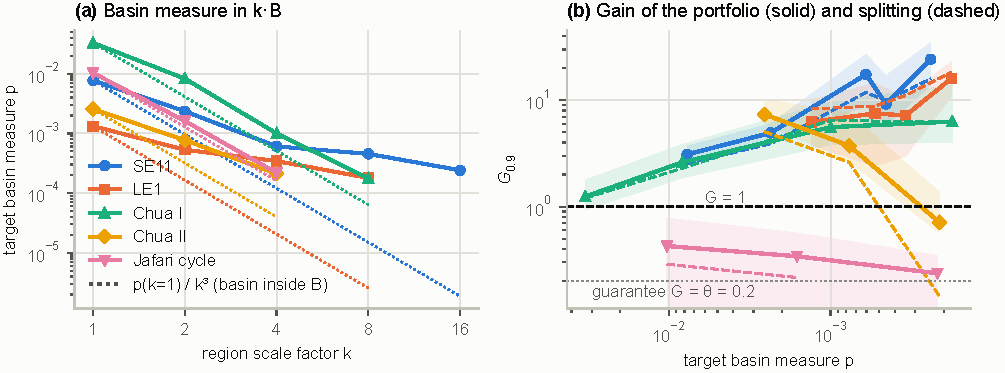
\includegraphics[width=\textwidth]{figures/fig27_enlarged_regions.pdf}
\caption{Real systems in enlarged regions $kB$. (a) Basin measure of the hidden target versus $k$; dotted lines: $p_{k=1}/k^3$, the measure if the basin lay inside $B$. (b) Gain of the portfolio (solid, with 95\% intervals) and of splitting (dashed) versus the basin measure, which decreases to the right. Dashed horizontal line: $G=1$; dotted: the guarantee $G=\theta=0.2$.}
\label{fig:enlarged}
\end{figure*}

\section{Discretization limit at very small \texorpdfstring{$p$}{p}}\label{app:smallp}

Figure~\ref{fig:smallp} shows the gain on D2 down to $p=10^{-7}$ and the diagnostic variants. Two alternative explanations of the breakdown below $p=10^{-5}$ were ruled out. Lowering the step floor of the splitting chains tenfold, or removing it, leaves every run unchanged: the floor is never reached. A second move that redraws a random subset of coordinates from the uniform distribution, akin to the componentwise Metropolis algorithm of the original subset simulation,\cite{AuBeck2001} helps only partly: at $p=10^{-6}$, splitting then succeeds in 50\% of runs and the portfolio in 68\%, but at $10^{-7}$ there is still no gain. The same move doubles the gain at $p=10^{-4}$ (53 for splitting and 35 for the portfolio); it is a natural extension of the method but is not used elsewhere in this paper. Reducing the integration step restores the order-of-growth gain, as stated in Sec.~\ref{sec:scaling_p}; these gains are counted in integrations, each of which is 4 or 16 times longer, so the gain in computing time is correspondingly smaller; the test demonstrates the mechanism, not a practical speedup. The level threshold also explains why one informative point is not enough: the level $\xi_l$ is the tenth largest value in the reference sample, and when fewer than ten points are informative, the threshold is $\xi_l=0$ (all escapes at the first step tie), the selection is empty, and the chains restart; the gain at $p=10^{-5}$ is carried by the runs whose reference sample contains several informative points. Figure~\ref{fig:scaln} shows the dependence on dimension at fixed $p=10^{-4}$.

\begin{figure}
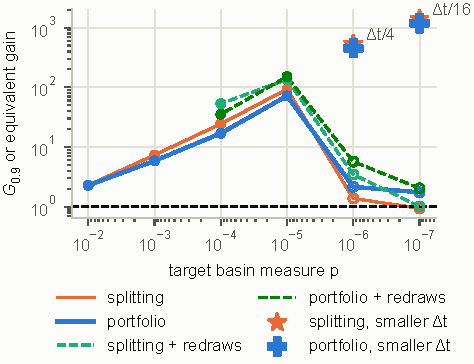
\includegraphics[width=\columnwidth]{figures/fig29_d2_small_p.pdf}
\caption{Family D2 ($n=6$): gain down to $p=10^{-7}$. Filled markers: $G_{0.9}$; open markers: equivalent gain $-\ln(1-f)/(pN_{\max})$ from the fraction $f$ of runs that found the target within the budget $N_{\max}$. Dashed lines: the variant with an additional move that redraws a random subset of coordinates (the variants with a lowered step floor coincide with the base curves and are not shown). Stars and crosses: splitting and the portfolio with the integration step reduced 4 times ($p=10^{-6}$) and 16 times ($p=10^{-7}$), with $N^0_{0.9}=\ln10/p$.}
\label{fig:smallp}
\end{figure}

\begin{figure}
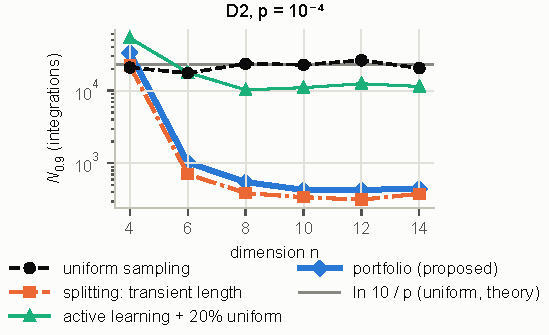
\includegraphics[width=\columnwidth]{figures/fig24_scaling_n.pdf}
\caption{Detection cost versus the phase-space dimension (family D2, $p=10^{-4}$, $R=100$). Dashed line: $\ln10/p$. At $n=4$, the reaction coordinate is uninformative because of the discretization limit; for $n\ge6$, the portfolio gain is 17--61 times.}
\label{fig:scaln}
\end{figure}

\section{Channel diagnostics}\label{app:diagnostics}

The prediction of the cost model was tested on a uniform sample of $2\times10^4$ points per system (Fig.~\ref{fig:signal}). Channel B works when nontarget points with long transients converge spatially to the target. For Chua~II, the median distance $d(q)$ decreases with the upper-set fraction $q$ as $0.43\to0.19\to0.12$; for LE1, as $0.53\to0.22\to0.13$; for SE11, as $0.47\to0.19\to0.15$; and for D2, as $0.74\to0.60\to0.53$ (at $q=0.2$, 0.04, and 0.008); the splitting gain here is 2.5--8.3 times. For the Jafari cycle ($0.99\to1.35$) and for D1 ($1.26\to1.38\to1.41$), $d(q)$ grows, and there is no gain. At the same time, in D1, the fraction of the target in the upper sets grows: the regions of long trajectories are scattered, and there is no path to the target through them. The AUC of the coordinate $\xi$ alone (0.88--0.97 for all systems except the Jafari cycle, 0.61) does not separate these cases, whereas $d(q)$ does. For the Huynh map, there is a gradient over only one decade ($d$ drops to 0.22 and grows again); at $p\approx0.009$, it barely pays back the initial sample and the levels.

\begin{figure}
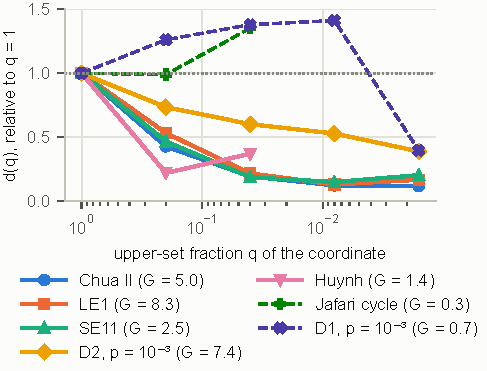
\includegraphics[width=\columnwidth]{figures/fig26_signal_curves.pdf}
\caption{Diagnostics of channel B from a uniform sample: the median distance from nontarget points of the upper set of the coordinate $\xi$ to the target (normalized to the value at $q=1$) versus the fraction $q$, which decreases to the right. A decreasing $d(q)$ (solid: Chua~II, LE1, SE11, D2) comes with a splitting gain (Tables~\ref{tab:gains} and \ref{tab:scaling}), and an increasing one (dashed: Jafari cycle, D1) with its absence.}
\label{fig:signal}
\end{figure}

\section{Implementation details of the two-stage configuration}\label{app:implementation}

The own computations of the arms (nearest-neighbor queries of the active-learning arm, the chains, and the matching) take 1--8\% of the wall time on the Chua systems with up to two copies, 28\% on three uncoupled copies of Chua~II, and 20--60\% on the cheap problems, where an integration costs microseconds. Brute-force neighbor search for $n\ge6$ reduces the queries by a factor of 1.6--2.6 relative to a tree ($G_T$ from 16 to 29 on three coupled copies of SE11). The cap on the training sample of the classifier (the last $2\times10^4$ evaluated points) removes the growth of the overhead in long runs: on three uncoupled copies of Chua~II, it lowers the overhead from 51\% to 28\% and, by training the classifier on recent points only, also lowers the median cost from $1.4\times10^5$ to $8.6\times10^4$ integrations and raises the number of runs that succeed within $4\times10^5$ integrations from 8 to 9 of 10. A wider batch, with two or four times more chains and boundary points to occupy more cores, does not pay: the number of evaluations grows by a factor of 1.5--3, whereas the time per evaluation decreases by about 10\% only. The gains in time of Table~\ref{tab:cost} were measured with four threads per process and those of Table~\ref{tab:time} on one thread; with the batch of 500 evaluations used here, the portfolio parallelizes better than uniform sampling (its time to detection falls 4.0-fold from one to four threads on the coupled Chua circuits, against 1.6-fold for the cost per uniform evaluation), so the four-thread gains are larger, and the one-thread values are the conservative ones.


\clearpage   % place all remaining figures before the reference list
\bibliography{refs}

\end{document}
